

% \section{Introduction}

% \section{ARIMA-Noise Models}



% $$y_{ti} = u_t + \epsilon_{ti}, \hspace{.4in} t=1,...T \hspace{.4in} i = 1,...,n \hspace{.4 in} \epsilon_{ti} \sim \text{i.i.d. } N(0,\sigma_\epsilon^2) $$

% $$u_t - \phi u_{t-1} = \eta_t + \theta\eta_{t-1}, \hspace{.4in} |\phi| < 1 \hspace{.2in} |\theta| < 1 \hspace{.2in} \eta_t \sim N(0,\sigma_\eta^2) $$

% $$\mathbf{y} = X_t\mathbf{u} + \mathbf{\epsilon} \hspace{.5in} \text{Var}(\mathbf{u}) = \Gamma = \sigma_\eta^2V\hspace{.5in} \text{Var}(\mathbf{y}) = X_t\Gamma X_t' + \sigma_\epsilon^2I $$

% \[X_t = \begin{bmatrix}
%     \mathbf{1}_n & 0           & 0 \\
%     0            & \ddots      & 0 \\
%     0            & 0           & \mathbf{1}_n
% \end{bmatrix}\]



% $\mathbf{w} = n^{-1}X_t'\mathbf{y} = \mathbf{u} + n^{-1}X_t'\epsilon$ is an ARMA-Noise Process, and therefore also an ARMA(1,1) process, with innovations $\{\nu_t\}_{t=1}^T$ and parameters $\{\phi,\theta_b,\sigma_b^2\}$

% Let $\hat{\phi}, \hat{\theta}_b, \hat{\sigma}_b^2$ be maximum likelihood estimators for $\phi,\theta,\sigma_b^2$.  

% $$\mathbf{y} \text{ is the vector of observed values, while } \mathbf{w}^{(0)} = n^{-1}X_t'\mathbf{y} - \hat{\beta}_0^{(0)}\text{ and }\mathbf{x} = \mathbf{y} - X_t\mathbf{w}$$

% Consider the observed process
% \begin{equation}
%     w_t = y_t + a_t, \qquad 
% a_t = n^{-1}\sum_{i=1}^n \varepsilon_{ti} \label{eq:arman}
% \end{equation}

% where the latent process $\{y_t\}$ follows an ARMA(1,1)
% \[
% y_t = \phi y_{t-1} + \eta_t + \theta \eta_{t-1}, 
% \qquad \eta_t \sim \text{i.i.d. } (0,\sigma_\eta^2),
% \]
% and $\varepsilon_{ti} \sim \text{i.i.d. } (0,\sigma_\varepsilon^2)$.
% Then $\bar{\varepsilon}_t$ has variance $\sigma_a^2 = \sigma_\varepsilon^2/n$.

% \medskip

% The observed process $\{w_t\}$ is itself ARMA(1,1) with parameters
% $(\phi,\theta_b,\sigma_b^2)$, so that
% \[
% w_t = \phi w_{t-1} + b_t + \theta_b b_{t-1}, 
% \qquad b_t \sim \text{i.i.d. } (0,\sigma_b^2).
% \]
% The autoregressive coefficient $\phi$ is common to both the latent and observed models. 
% Hence only $(\theta,\sigma_\eta^2)$ must be estimated for the latent process.

% \subsection*{How Noise Alters an ARMA(1,1) Process}

% $$w_t = y_t + a_t \qquad y_t - \phi y_{t-1} = \eta_t + \theta\eta_{t-1} \qquad \eta_t \sim \text{i.i.d. }N(0,\sigma_\eta^2) \qquad a_t \sim \text{i.i.d. } N(0,\sigma_\varepsilon^2/n) $$

% $$ \gamma_x(h) := \text{Cov}(X_t, X_{t+h}) \qquad \gamma_w(h) = \gamma_y(h) + \gamma_a(h) $$

% $$ \gamma_w(0) = \sigma_\eta^2(1 + \frac{(\phi + \theta)^2}{1 - \phi^2}) + \frac{\sigma_\varepsilon^2}{n} $$

% $$ \gamma_w(1) = \sigma_\eta^2(\phi + \theta + \frac{\phi(\phi + \theta)^2}{1 - \phi^2}) $$

% From Wong and Miller (1990), we know that $\{w_t\}$ is itself an ARMA(1,1) process parameterized by $\phi,\theta_b,\sigma_b^2$.

% \vspace{.2in}

% In seeking to express $\theta_b,\sigma_b^2$ in terms of $\phi, \theta, \sigma_\varepsilon^2,\sigma_\eta^2,n$, we obtain the following system of equations:

% $$ \sigma_b^2(1 + \frac{(\phi + \theta_b)^2}{1 - \phi^2}) = \sigma_\eta^2(1 + \frac{(\phi + \theta)^2}{1 - \phi^2}) + \frac{\sigma_\varepsilon^2}{n} $$

% $$ \sigma_b^2(\phi + \theta_b + \frac{\phi(\phi + \theta_b)^2}{1 - \phi^2}) = \sigma_\eta^2(\phi + \theta + \frac{\phi(\phi + \theta)^2}{1 - \phi^2}) $$

% If we define the following intermediate functions:

% $$ a = \phi + \theta, \qquad b = \phi + \theta_b, \qquad c = 1 - \phi^2, \qquad d = \frac{\sigma_\varepsilon^2}{n\sigma_\eta^2} $$


% We obtain:

% $$ \sigma_b^2\left[1 + \frac{b^2}{c}\right] = \sigma_\eta^2 \left[ 1 + \frac{a^2}{c} + d \right] $$

% $$ \sigma_b^2\left[ b + \frac{\phi b^2}{c} \right] = \sigma_\eta^2\left[ a + \frac{\phi a^2}{c} \right] $$

% Solving for $\sigma_b^2$ in the second equation and substituting it out of the first, we arrive at:

% $$ \left[ 1 + \frac{a^2}{c} + d \right] \left[ b + \frac{\phi b^2}{c} \right] = \left[ a + \frac{\phi a^2}{c} \right] \left[ 1 + \frac{b^2}{c} \right] $$


% Combining like terms in order to solve a quadratic equation for b, we obtain:

% \[
% b^2 \underbrace{\left[ \frac{\phi}{c} + \frac{\phi d}{c} - \frac{a}{c} \right]}_{e}
% + b \underbrace{\left[ 1 + \frac{a^2}{c} + d \right]}_{f}
% + \underbrace{\left[ -a - \frac{\phi a^2}{c} \right]}_{g}
% = 0
% \]

% Solving for b and subtracting $\phi$ gives solutions for $\theta_b$. Empirical results suggest that it is only $\frac{-f + \sqrt{f^2 - 4eg}}{2e}$ that yields a valid result, namely a value for $\theta_b$ of norm less than 1.

% Substituting $\theta_b$ into the original system of equations allows us to solve for $\sigma_b^2$, enabling us to get a sense of how added noise changes the MA and variance parameters of an ARMA(1,1) process:

% \vspace{.5in}

% 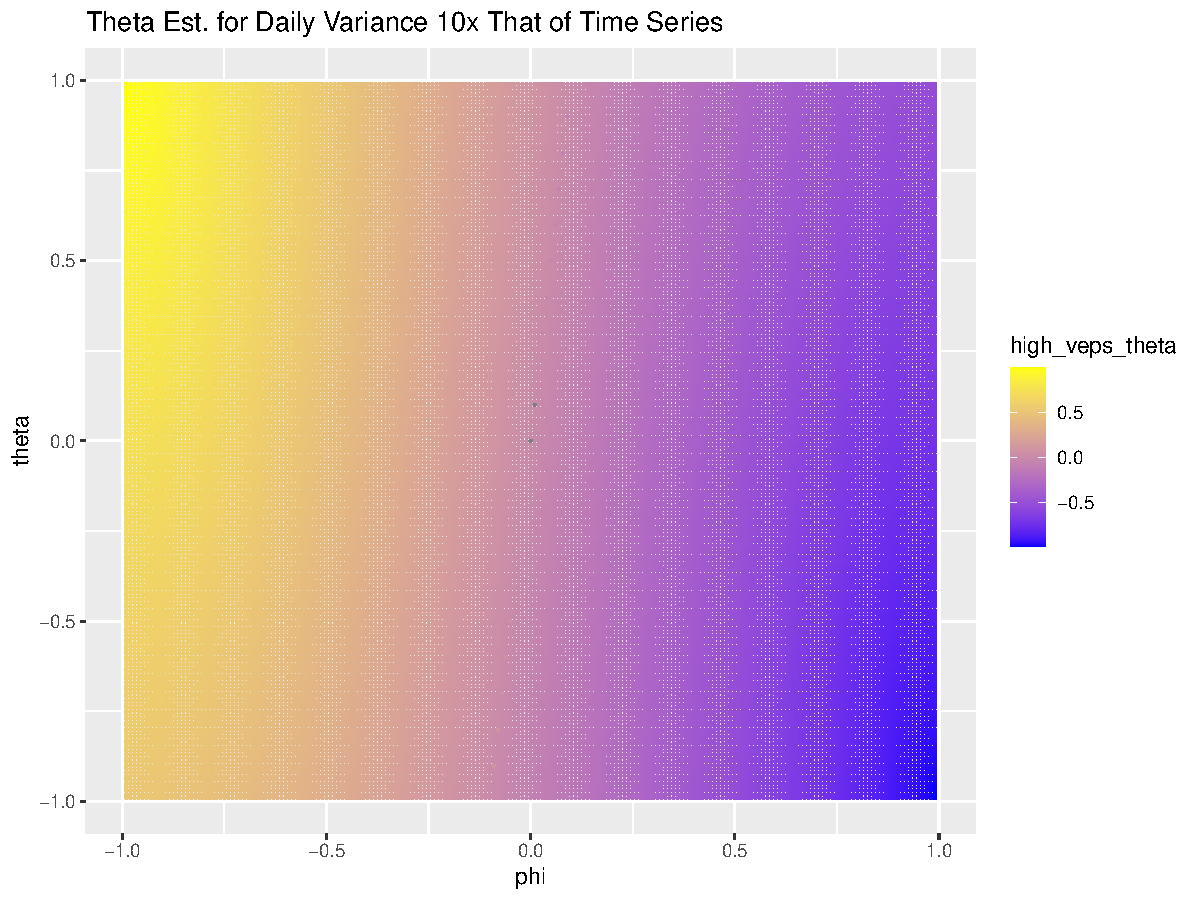
\includegraphics[width = .7\linewidth]{images/output/high_veps.pdf}

% 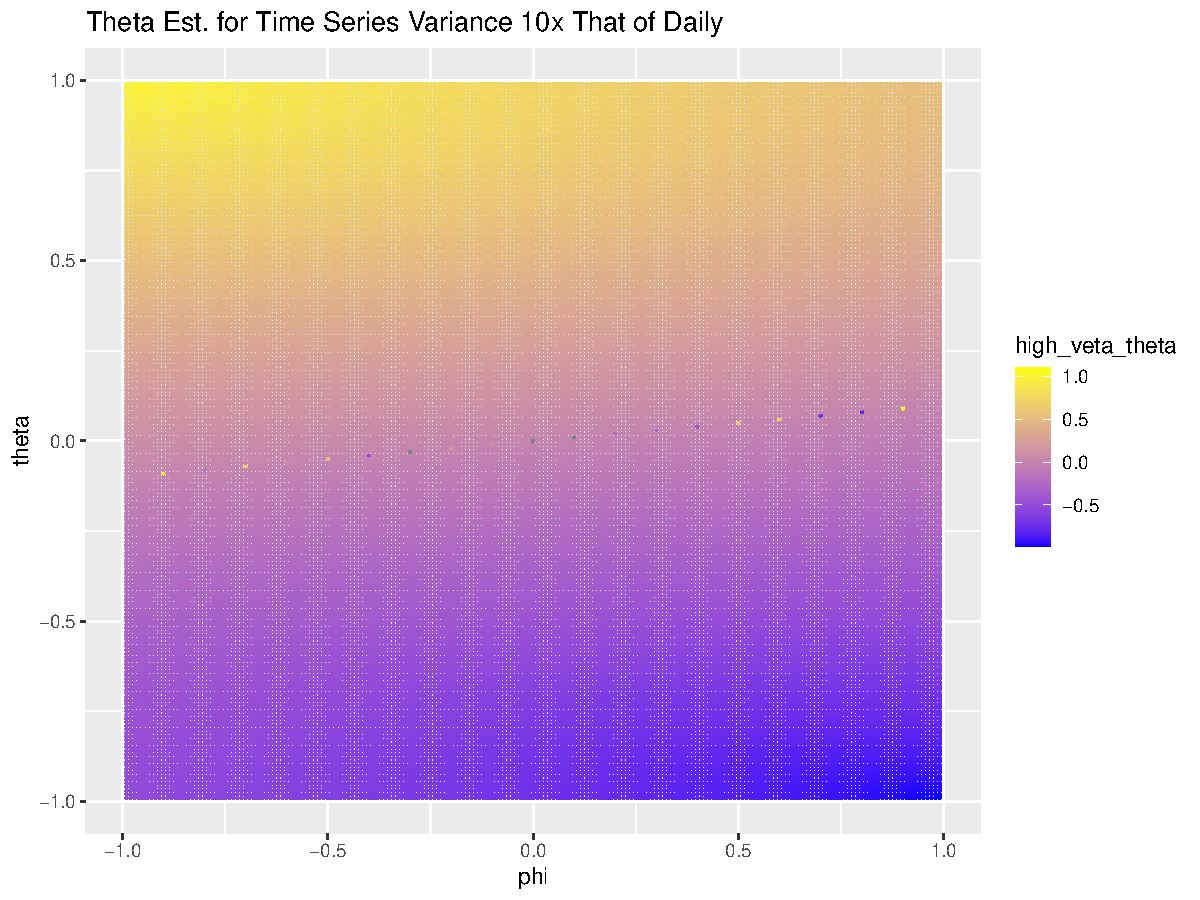
\includegraphics[width = .7\linewidth]{images/output/high_veta.pdf}

% 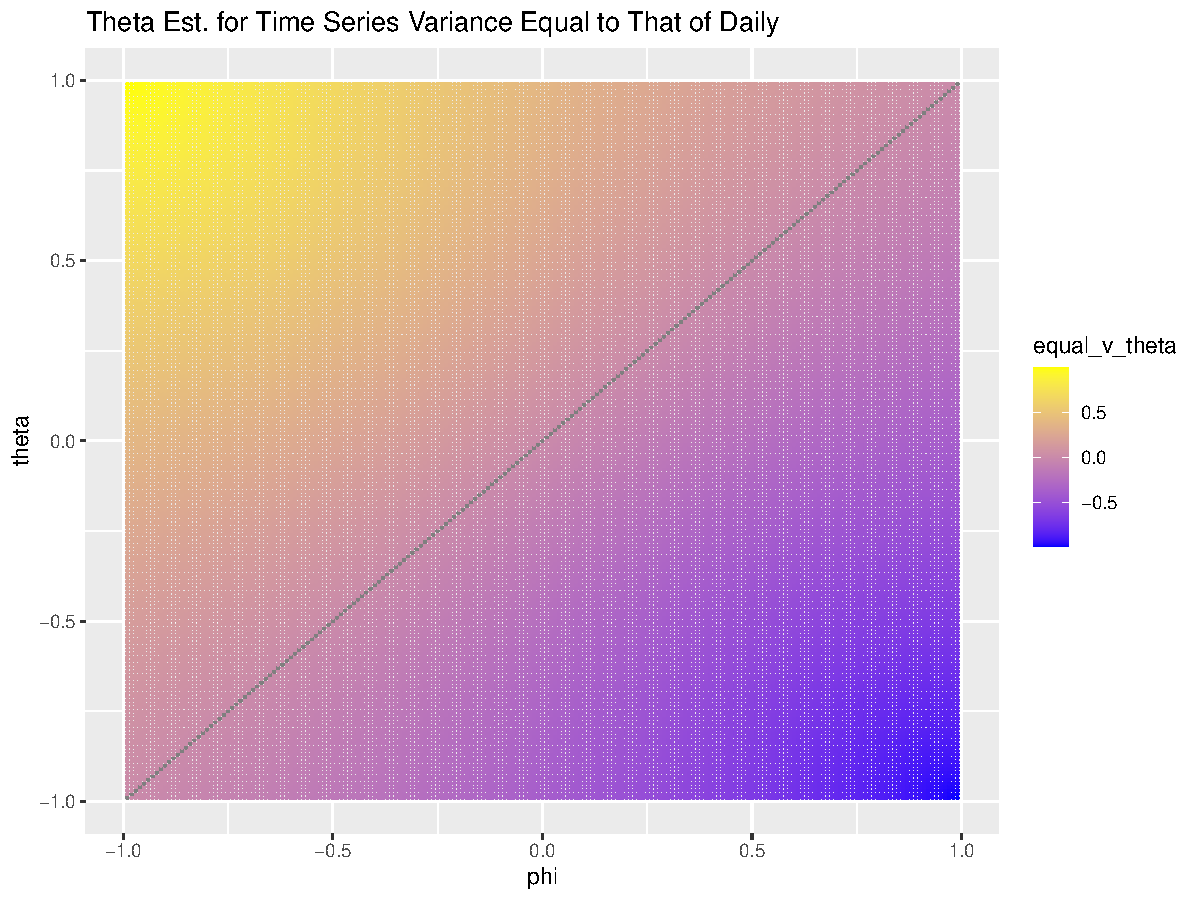
\includegraphics[width = .7\linewidth]{images/output/equal_v.pdf}

% 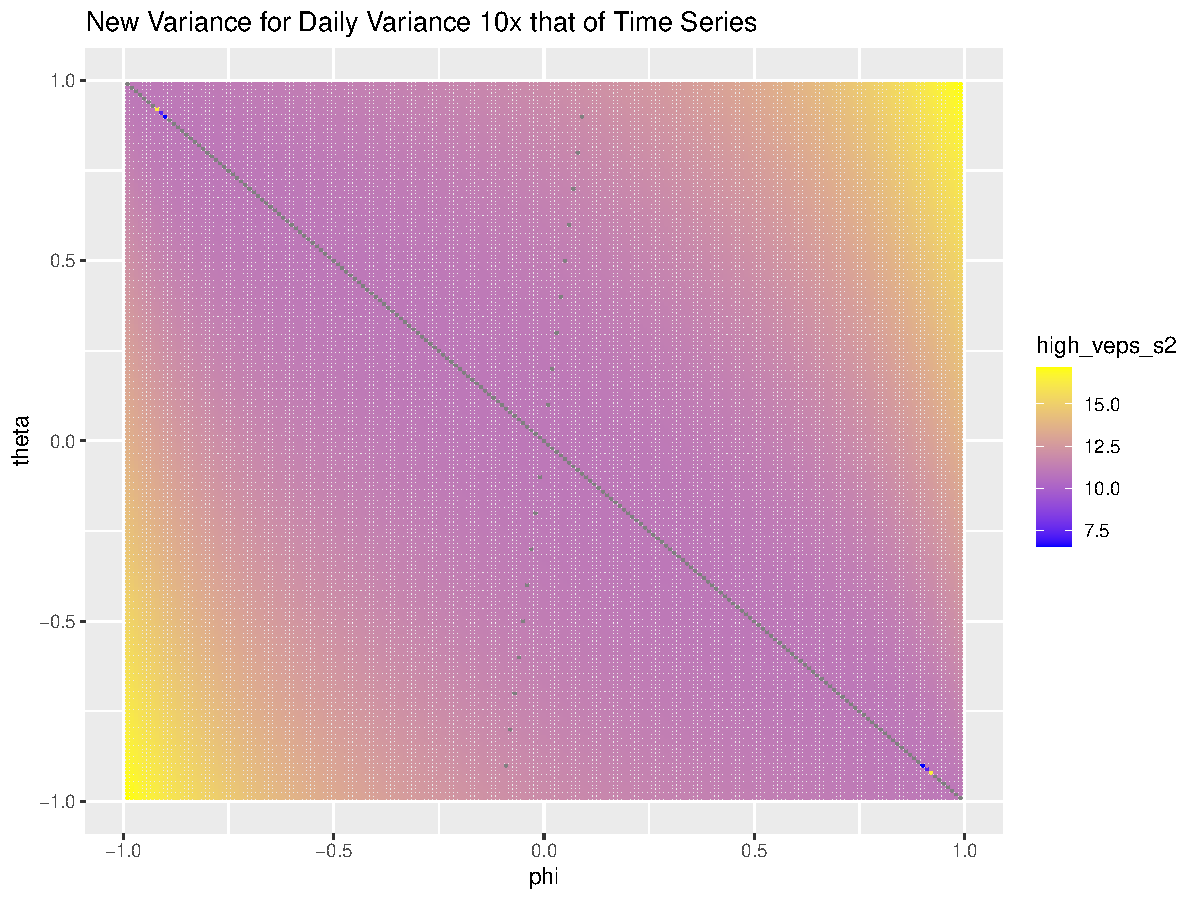
\includegraphics[width = .7\linewidth]{images/output/high_veps_s2.pdf}

% 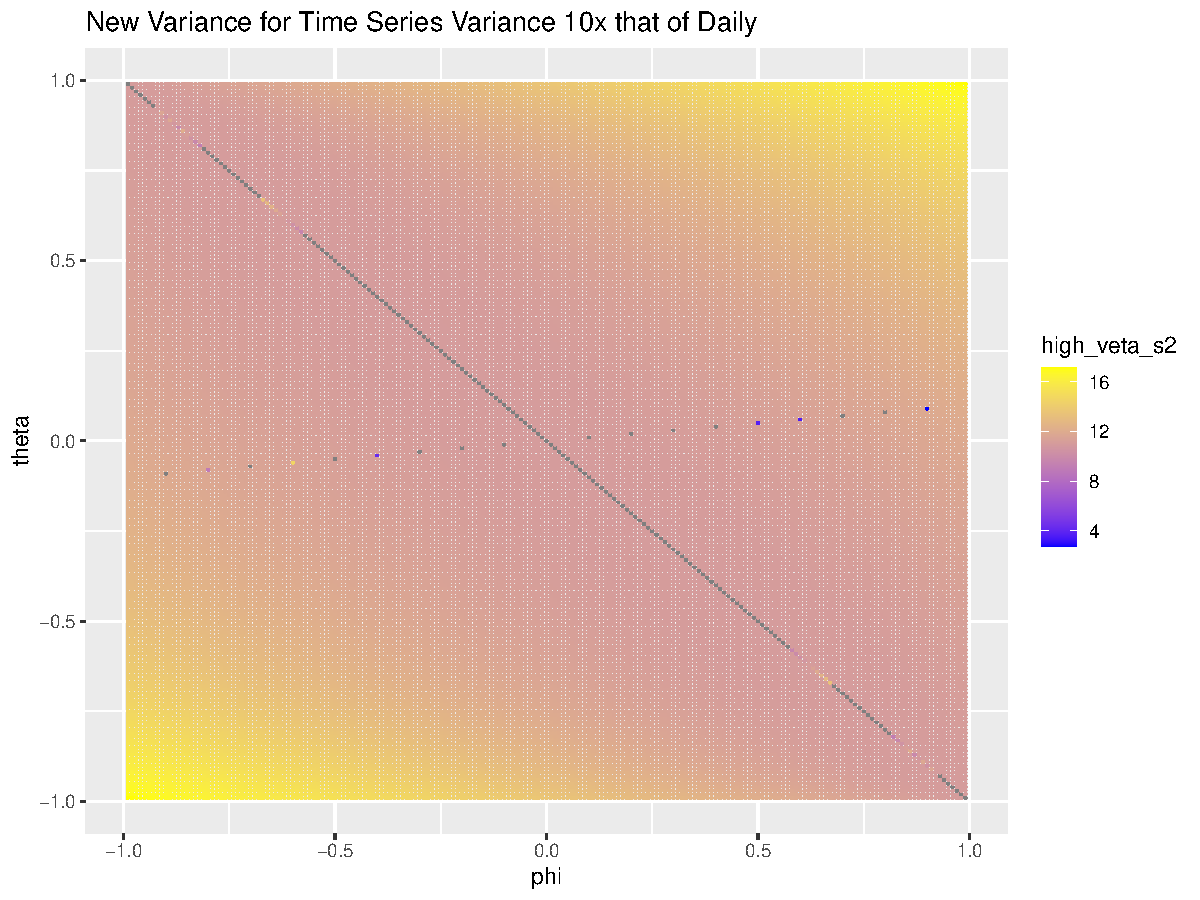
\includegraphics[width = .7\linewidth]{images/output/high_veta_s2.pdf}

% 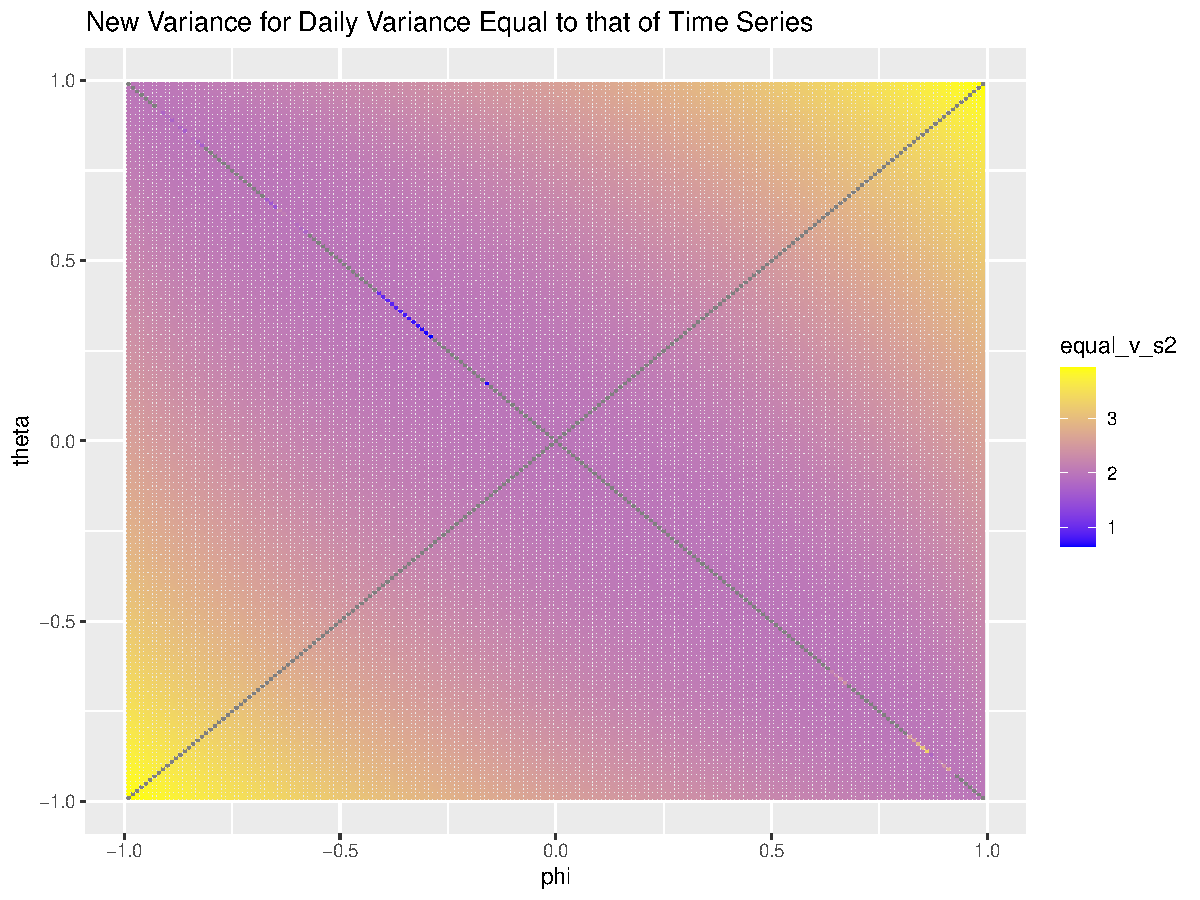
\includegraphics[width = .7\linewidth]{images/output/equal_v_s2.pdf}


% \subsection*{Relating Autocovariance Functions}

% Let B denote the backward operator. We can then express Equation 1 as:

% $$ (1 - \phi B)y_t = (1+\theta B)\eta_t $$

% So long as $|\phi| < 1$, we can give an explicit expression for $y_t$:

% $$ y_t = (1-\phi B)^{-1}(1 + \theta B)\eta_t $$

% Doing the same with $w_t$ in \ref{eq:arman}, we obtain the following:

% $$ (1 - \phi B) ^ {-1} (1 + \theta_b B) b_t =  (1 - \phi B) ^ {-1} (1 + \theta B) \eta_t + a_t $$

% Left multiplying $(1 - \phi B)$ to both sides gives us:

% $$ (1 + \theta_b B) b_t = (1 + \theta B) \eta_t + (1 - \phi B) a_t $$

% This is now a relation between three independent MA(1) processes: $\{\nu_{b,t}\}, \{\nu_{\eta,t}\}, \{\nu_{a,t}\}$. From their independence we obtain the following system of equations relating their respective auto-covariance functions at lags 0 and 1:

% $$H(\theta,\sigma_\eta^2) = \begin{cases}
%         \gamma_{\nu,\eta}(i) + \gamma_{\nu,a}(i) - \gamma_{\nu,b}(i) \qquad i = 0,1
% \end{cases}$$

% This works out to: 
% \begin{equation}
%    H(\theta,\sigma_\eta^2) = \left( \begin{array}{c}
%         (1 + \theta^2)\sigma_\eta^2 + (1  + \phi^2)\sigma_a^2 - (1 + \theta_b^2)\sigma_b^2 \\
%         \theta\sigma_\eta^2 -\phi\sigma_a^2 - \theta_b\sigma_b^2
%     \end{array} \right) = \mathbf{0}
%     \label{eq:H}
% \end{equation}

% \[
% F(\theta,\sigma_\eta^2;\mathbf{u}_2) = H(\theta,\sigma_\eta^2) \text{,
% where }\mathbf{u}_2 = (\phi,\theta_b,\sigma_b^2,\sigma_a^2)'. \]

% \subsection*{Implicit Function Theorem Setup}

% Question for Professor: Why might Wong reduce the system of equations F by substituting out $\sigma_\eta^2$ if that is a parameter of interest?

% Let $\bm{\tau} = (\theta,\sigma_\eta^2)'$ and suppose
% $F(\bm{\tau},\mathbf{u}_2) = \bm{0}$ defines $\bm{\tau} = g(\mathbf{u}_2)$ locally.
% Then, by the Implicit Function Theorem,
% \[
% G = \frac{\partial \bm{\tau}}{\partial \mathbf{u}_2}
% = -\left(\frac{\partial F}{\partial \bm{\tau}}\right)^{-1}
%   \left(\frac{\partial F}{\partial \mathbf{u}_2}\right).
% \]
% The required partial derivatives are given below.

% \paragraph{(i) With respect to $\bm{\tau} = (\theta,\sigma_\eta^2)$:}
% \[
% \frac{\partial F}{\partial \bm{\tau}}
% =
% \begin{pmatrix}
%  2\theta\sigma_\eta^2 & (1 + \theta^2) \\[4pt]
%  \sigma_\eta^2 & \theta
% \end{pmatrix}.
% \]

% \paragraph{(ii) With respect to $\mathbf{u}_2 = (\phi,\theta_b,\sigma_b^2,\sigma_\nu^2)$:}
% \[
% \frac{\partial F}{\partial \mathbf{u}_2}
% =
% \begin{pmatrix}
% 2\phi\sigma_a^2
% & -2\theta_b\sigma_b^2
% & -(1 + \theta_b^2)
% & (1 + \phi^2)\\[4pt]
% -\sigma_a^2
% & -\sigma_b^2
% & -\theta_b
% & -\phi
% \end{pmatrix}.
% \]

% \subsection*{Asymptotic Covariance of $(\hat\theta,\widehat\sigma_\eta^2)$}
% From Brockwell and Davis we have the following:
% $$ \sqrt{T}\left( \left[ \begin{array}{cc}
%     \hat{\phi} \\
%     \hat{\theta}_b
% \end{array}\right] - \left[ \begin{array}{cc}
%     {\phi} \\
%     {\theta_b}
% \end{array}\right] \right) \xrightarrow{d} N(\mathbf{0},\Sigma), \qquad \Sigma =  \frac{1 + \phi \theta_b}{(\phi + \theta_b)^2} \left[ \begin{array}{cc}
%     (1 - \phi^2)(1 + \phi\theta_b) & -(1 - \theta_b^2)(1 - \phi^2) \\
%     -(1 - \theta_b^2)(1 - \phi^2) & (1 - \theta_b^2)(1 + \phi\theta_b)
% \end{array} \right] $$

% Let $\mathbf{u}_{20}$ denote the true value of $\mathbf{u}_2$, and assume
% \[
% \sqrt{T}(\widehat{\mathbf{u}}_2 - \mathbf{u}_{20})
% \xrightarrow{d} N(\mathbf{0},\Sigma_1).
% \]
% Then by the multivariate delta method,
% \[
% \sqrt{T}(\widehat{\bm{\tau}} - \bm{\tau})
% \xrightarrow{d} N(\mathbf{0},\Sigma_\tau),
% \qquad
% \Sigma_\tau = G\,\Sigma_1\,G'.
% \]





% \section{$\mu$-mean ARIMA}
% \section{$\mu$-mean ARIMA-Noise}

% $$y_{ti} = \beta_0 + u_t + \epsilon_{ti}, \hspace{.4in} t=1,...T \hspace{.4in} i = 1,...,n \hspace{.4 in} \epsilon_{ti} \sim N(0,\sigma_\epsilon^2) $$

% $$u_t - \phi u_{t-1} = \eta_t + \theta\eta_{t-1}, \hspace{.4in} |\phi| < 1 \hspace{.2in} |\theta| < 1 \hspace{.2in} \eta_t \sim N(0,\sigma_\eta^2) $$

% $$\mathbf{y} = \beta_0 + X_t\mathbf{u} + \mathbf{\epsilon} \hspace{.5in} \text{Var}(\mathbf{u}) = \Gamma = \sigma_\eta^2V\hspace{.5in} \text{Var}(\mathbf{y}) = X_t\Gamma X_t' + \sigma_\epsilon^2I $$

% \[X_t = \begin{bmatrix}
%     \mathbf{1}_n & 0           & 0 \\
%     0            & \ddots      & 0 \\
%     0            & 0           & \mathbf{1}_n
% \end{bmatrix}\]

% $$\hat{\beta}_0 = \bar{\mathbf{y}} $$

% $$\text{Var}(\hat{\beta}_0) = \frac{\sigma_\epsilon^2}{N} + \frac{\sigma_\eta^2}{T^2}(\mathbf{1}')V (\mathbf{1}) $$

% $$\text{For an MA(1) model: Var} (\hat{\beta}_0) = (N)^{-1}\sigma_\epsilon^2 + (T)^{-2}(T(1+\theta^2)+2(T-1)\theta) \sigma_\eta^2$$

% $$\hat{\mathbf{u}}^{(0)} = \bar{\mathbf{y}}$$

% $\mathbf{v}:= \mathbf{u} + n^{-1}X_t'\epsilon$ is an ARIMA-Noise process, whereas $\mathbf{w} = n^{-1}X_t'\mathbf{y} - \hat{\beta}_0 = \mathbf{u} + n^{-1}X_t'\epsilon + c$,  in which $c$ is a constant with variance equal to that of $\beta_0$

% $$\mathbf{y} \text{ is the vector of observed values, while } \mathbf{w}^{(0)} = n^{-1}X_t'\mathbf{y} - \hat{\beta}_0^{(0)}\text{ and }\mathbf{x} = \mathbf{y} - X_t\mathbf{w}$$



% \section{Simple Linear Model}

% \vspace{.1in}

% $$y_{ti} = \beta_0 + u_t + \epsilon_{ti}, \hspace{.4in} t=1,...T \hspace{.4in} i = 1,...,n \hspace{.4 in} \epsilon_{it} \sim N(0,\sigma_\epsilon^2) $$

% $$u_t - \phi u_{t-1} = \eta_t + \theta\eta_{t-1}, \hspace{.4in} |\phi| < 1 \hspace{.2in} |\theta| < 1 \hspace{.2in} \eta_t \sim N(0,\sigma_\eta^2) $$

% $$Var(\mathbf{y}) = X_t\Gamma X_t' + \sigma_\epsilon^2I $$



% \[X_f = (\begin{array}{cc}
%     \mathbf{1} & X_t\mathbf{t}
% \end{array}) \hspace{.5in} \mathbf{t} = (1,...,T)'\hspace{.5in} X_t = \begin{bmatrix}
%     \mathbf{1}_n & 0           & 0 \\
%     0            & \ddots      & 0 \\
%     0            & 0           & \mathbf{1}_n
% \end{bmatrix}\]

% $$\hat{\beta} = (X_f'X_f)^{-1}X_f'\mathbf{y} $$

% $$Var(\hat{\beta}) = (X_f'X_f)^{-1}\sigma_\epsilon^2 + (X_f'X_f)^{-1} X_f'(X_t\Gamma X_t)X_f(X_f'X_f)^{-1} $$

% $$X_f'X_f = \begin{bmatrix}
%     N & \frac{N(T+1)}{2} \\
%     \frac{N(T+1)}{2} & \frac{N(T+1)(2T+1)}{6}
% \end{bmatrix}$$

% $$(X_f'X_f)^{-1} = \frac{12}{N} \begin{bmatrix}
%     \frac{(T+1)(2T+1)}{6} & \frac{-(T+1)}{2} \\
%     \frac{-(T+1)}{2} & 1
% \end{bmatrix}$$

% $$X_f'X_t = n\begin{bmatrix}
%     \mathbf{1} \\
%     \mathbf{t}
% \end{bmatrix}$$

% \section{Linear Regression}

% \section{Discussion}

% \section{Wong Working Paper}
% Property 2.1 adapts as follows:
% \[
% \{u_t\} \text{ is an ARIMA (1,0,1) process, whereas } \{a_t\} \text{ is an ARIMA(0,0,0) process.} 
% \]
% As such, $\{w_t = u_t + a_t\}$ is an ARIMA(p,d,q) process, in which $p = 1$, $d = 0$, and $q\leq 1$
% We adapt Section 3 of the working paper "Analysis of ARIMA-NOISE Models with Repeated Time Series" to our context, namely one with a first-order ARMA-Noise Model in which $p = q = 1$:

% \[
% F(\theta,\mathbf{u}_2) = f_1(\theta,\mathbf{u}_2)
% \]



% \[
% f_1(\theta) = \frac{\phi\sigma_a^2 + \theta_b\sigma_b^2}{\theta} + \theta\phi\sigma_a^2 + \theta\theta_b\sigma_b^2 + (1 + \phi^2)\sigma_a^2 - (1 + \theta_b^2)\sigma_b^2
% \]

% \[
% \mathbf{u}_1 = (\phi,\theta_b)', \qquad \mathbf{u}_2 = (\phi,\theta_b,\sigma_b^2,\sigma_a^2)
% \]

% Let $\theta_0$ denote the true MA parameter. Under conditions specified in Wong and Miller (1988): 

% $$\sqrt{T}(\hat{\theta} - \theta_0) \xrightarrow{d} N(\mathbf{0}, \Sigma_\theta)$$

% $$\Sigma_\theta = G_1(\mathbf{u_2}_0)\Sigma_1G_1(\mathbf{u_2}_0)'$$

% $$\Sigma_1 = \text{Cov}(\mathbf{u_2}, \mathbf{u_2})$$

% $$G_1 = \left[ \frac{\partial g_l}{\partial u_k} \right]_{q \times t} = -\left[ \frac{\partial f_i}{\partial \theta_j} \right]^{-1}_{q \times q} \left[ \frac{\partial f_l}{\partial u_k} \right]_{q \times t} $$

% $$ G_1 \Sigma_1 G_1' = \sum_{i = a,b} \text{Var}(\hat{\sigma}_i^2) \left[ \frac{\partial G}{\partial \sigma_i^2}\right] \left[ \frac{\partial G}{\partial \sigma_i^2}\right]^T + G_2\Sigma G_2', \qquad G_2 = \left[ \frac{\partial g_i}{\partial u_j}  \right]_{q \times s} $$

% In an ARMA-Noise(1,1) we obtain the following: 
% $$ \frac{\partial f_1}{\partial \theta} = -\theta^{-2} (\phi\sigma_a^2 + \theta_b\sigma_b^2) + \phi \sigma_a^2 + \theta_b\sigma_b^2 = (1 - \theta^{-2})(\phi\sigma_a^2 + \theta_b\sigma_b^2) $$

% $$ \frac{\partial f_1}{\partial \phi} = \theta^{-1} \sigma_a^2 + \theta\sigma_a^2 + 2\phi\sigma_a^2  = (\theta^{-1} + \theta + 2\phi)\sigma_a^2 $$

% $$ \frac{\partial f_1}{\partial \theta_b} = \theta^{-1} \sigma_b^2 + \theta \sigma_b^2 - 2\theta_b\sigma_b^2 = (\theta^{-1} + \theta -2\theta_b)\sigma_b^2 $$

% $$ \frac{\partial f_1}{\partial \sigma_b^2} = \theta^{-1}\theta_B + \theta\theta_b - (1+\theta_b^2) $$

% $$ \frac{\partial f_1}{\partial \sigma_a^2} = \theta^{-1}\phi + \theta\phi + 1 + \phi^2 $$


% \section{Reconfiguring Likelihood Function}


% We start with the following expression for the likelihood function $L(\xi|\mathbf{y})$:

% $$ L(\xi|\mathbf{y}) = (2\pi)^{-N/2}|\Omega|^{-1/2}\exp{(-\frac{1}{2})\mathbf{y}'\Omega^{-1}}\mathbf{y} $$

% $$ L_b(\xi_b|\mathbf{w}) = (2\pi)^{-N/2}|\Gamma_b|^{-1/2}\exp{(-\frac{1}{2})\mathbf{w}'\Gamma_b^{-1}}\mathbf{w} $$

% From Brockwell and Davis 1987, we can express the above equation as:

% $$ L(\phi,\theta_b,\sigma_b^2) = (2\pi\sigma_b^2)^{-T/2}(r_0...r_{T-1})^{-1/2}\exp{\left[ -\frac{1}{2}\sigma_b^2\sum_{j=1}^T(w_j -\hat{w}_j)^2/r_{j-1} \right]} $$

% This is based on applying the Innovations Algorithm (Proposition 5.2.2 from the same text). From this we get the following expressions for our maximum likelihood estimates:

% $$ \hat{\sigma}_b^2 = T^{-1} S(\hat{\phi}, \hat{\theta}) \qquad S(\hat{\phi}, \hat{\theta}) = \sum_{j=1}^T (w_j - \hat{w}_j)^2/r_{j-1} $$

% $$ l(\phi,\theta,\sigma_b^2|\mathbf{w}) = \frac{-T}{2}\text{ln}(2\phi\sigma_b^2) - \frac{1}{2}\sum_{j=0}^{T-1}\text{ln}(r_j) - \frac{1}{2}\sigma_b^{-2}\sum_{j=1}^T (w_j - \hat{w}_j)^2/r_{j-1}  $$

% $$ \frac{\partial l}{\partial \sigma_b^2} = -\frac{T}{2\sigma_b^2} + \frac{1}{2\sigma_b^4}\sum_{j=1}^T (w_j - \hat{w}_j)^2/r_{j-1}$$

% $$ \frac{\partial^2 l}{\partial \sigma_b^4} = \frac{T}{2\sigma_b^4} - \frac{1}{\sigma_b^6}\sum_{j=1}^T (w_j - \hat{w}_j)^2/r_{j-1}$$

% From 8.7.3 of Brockwell and Davis we obtain the expectation of the above expression, which we negate to find the Fischer Information:

% $$ I(\sigma_b^2) = -\mathbb{E}\left(\frac{\partial^2 l}{\partial \sigma_b^4}\right) = -\mathbb{E}\left(\frac{T}{2\sigma_b^4} - \frac{1}{\sigma_b^6}\sum_{j=1}^T (w_j - \hat{w}_j)^2/r_{j-1}\right) = \frac{T}{2\sigma_b^4} $$



% The relative simplicity of these derivative expressions are justified on page 256 of Brockwell and Davis, which states that $\{ (w_j-\hat{w_j})^2\}_{j=1}^T$ and $\{r_j\}_{j=1}^T$ are independent of $\sigma_b^2$.
% \bibliography{bib}

% In seeking the offdiagonal terms of the asymptotic variance matrix, we give the following expressions:

% $$  \frac{\partial^2 l}{\partial \sigma_b^2 \partial \phi} = \frac{1}{2\sigma_b^4} \frac{\partial}{\partial \phi} \left[ \sum_{j=1}^T (w_j - \hat{w}_j)^2/r_{j-1}\right] $$

% $$  \frac{\partial^2 l}{\partial \sigma_b^2 \partial \theta_b} = \frac{1}{2\sigma_b^4} \frac{\partial}{\partial \theta_b} \left[ \sum_{j=1}^T (w_j - \hat{w}_j)^2/r_{j-1}\right] $$


% $$ \frac{\partial}{\partial \phi}\frac{(w_j-\hat{w}_j)^2}{r_{j-1}} = (-2(w_j - \hat{w}_{j-1})\frac{\partial}{\partial\phi}r_{j-1} - (w_j - \hat{w}_j)^2\frac{\partial}{\partial\phi}r_{j-1})r_{j-1}^{-2} $$

% For the simplification of calculations, we leverage the use of a transformed process: 
% $$v_t = \begin{cases}
%     \sigma_b^{-1}w_t & t = 1,...,\text{max}(p,q) \\ \sigma_b^{-1}\phi(B)w_t & t > \text{max}(p,q)
    
% \end{cases}$$

% From page 177 we get: 
% $$ \begin{cases}
%     r_0 = (1 + 2\phi\theta_b + \theta_b^2)/(1-\phi^2), \\
%     \theta_{b,n1} = \theta_b/r_{n-1}, \\
%     r_n = 1 + \theta_b^2 - \theta_b^2/r_{n-1}
    
% \end{cases} $$


% \subsection*{How Noise Alters an ARMA(1,1) Process (Forward Direction):}
% \begin{equation}
%     \label{eq:arman}
%     w_t = u_t + a_t \qquad u_t - \phi u_{t-1} = \eta_t + \theta\eta_{t-1} \qquad \eta_t \sim \text{i.i.d. }N(0,\sigma_\eta^2) \qquad a_t \sim \text{i.i.d. } N(0,\sigma_\varepsilon^2/n)
% \end{equation}


% $$ \gamma_Z(h) := \text{Cov}(Z_t, Z_{t+h}) \qquad \gamma_w(h) = \gamma_y(h) + \gamma_a(h) $$

% \vspace{.2in}

% Given the explicit ACVF of an ARMA(1,1) process, we obtain the following:

% $$ \gamma_w(0) = \sigma_\eta^2 \left[1 + \frac{(\phi + \theta)^2}{1 - \phi^2}\right] + \frac{\sigma_\varepsilon^2}{n} \qquad \gamma_w(1) = \sigma_\eta^2\left[\phi + \theta + \frac{\phi(\phi + \theta)^2}{1 - \phi^2}\right] $$



% In seeking to express $\theta_b,\sigma_b^2$ as a function of parameters $(\phi, \theta, \sigma_\varepsilon^2,\sigma_\eta^2,n)$, we obtain the following system of equations:

% $$ \sigma_b^2\left[1 + \frac{(\phi + \theta_b)^2}{1 - \phi^2}\right] = \sigma_\eta^2\left[1 + \frac{(\phi + \theta)^2}{1 - \phi^2}\right] + \frac{\sigma_\varepsilon^2}{n} $$

% $$ \sigma_b^2\left[\phi + \theta_b + \frac{\phi(\phi + \theta_b)^2}{1 - \phi^2}\right] = \sigma_\eta^2\left[\phi + \theta + \frac{\phi(\phi + \theta)^2}{1 - \phi^2}\right] $$

% If we define the following intermediate functions:

% $$ a = \phi + \theta, \qquad b = \phi + \theta_b, \qquad c = 1 - \phi^2, \qquad d = \frac{\sigma_\varepsilon^2}{n\sigma_\eta^2} $$


% We obtain:

% $$ \sigma_b^2\left[1 + \frac{b^2}{c}\right] = \sigma_\eta^2 \left[ 1 + \frac{a^2}{c} + d \right] $$

% $$ \sigma_b^2\left[ b + \frac{\phi b^2}{c} \right] = \sigma_\eta^2\left[ a + \frac{\phi a^2}{c} \right] $$

% Solving for $\sigma_b^2$ in the second equation and substituting it out of the first, we arrive at:

% $$ \left[ 1 + \frac{a^2}{c} + d \right] \left[ b + \frac{\phi b^2}{c} \right] = \left[ a + \frac{\phi a^2}{c} \right] \left[ 1 + \frac{b^2}{c} \right] $$


% Combining like terms in order to solve a quadratic equation for b, we obtain:

% \[
% b^2 \underbrace{\left[ \frac{\phi}{c} + \frac{\phi d}{c} - \frac{a}{c} \right]}_{e}
% + b \underbrace{\left[ 1 + \frac{a^2}{c} + d \right]}_{f}
% + \underbrace{\left[ -a - \frac{\phi a^2}{c} \right]}_{g}
% = 0
% \]

% Solving for b and subtracting $\phi$ gives solutions for $\theta_b$. Empirical results suggest that it is only $\frac{-f + \sqrt{f^2 - 4eg}}{2e}$ that yields a valid result, namely a value for $\theta_b$ of norm less than 1.

% Substituting $\theta_b$ into the original system of equations allows us to solve for: $$\sigma_b^2 = \sigma_\eta^2 \left[ a + \frac{\phi a^2}{c} \right] \left[ b + \frac{\phi b^2}{c} \right]^{-1} $$

% \vspace{.5in}

% Having demonstrated that $(\theta_b, \sigma_b^2)$ is expressible as a function of $(\phi,\theta,\sigma_\eta^2, \sigma_a^2)$, we can explore how added noise impacts ARMA(1,1) processes with varying parameters. Of greater interest, however, is expressing $\theta$ and $\sigma_\eta^2$ (parameters of latent time series) as a function of $\phi,\theta_b,\sigma_b^2,\sigma_a^2$ (parameters of observed time series/deviations).
% \begin{figure}[h!]
%     \centering
%     \label{fig::armanoisefwd}
%     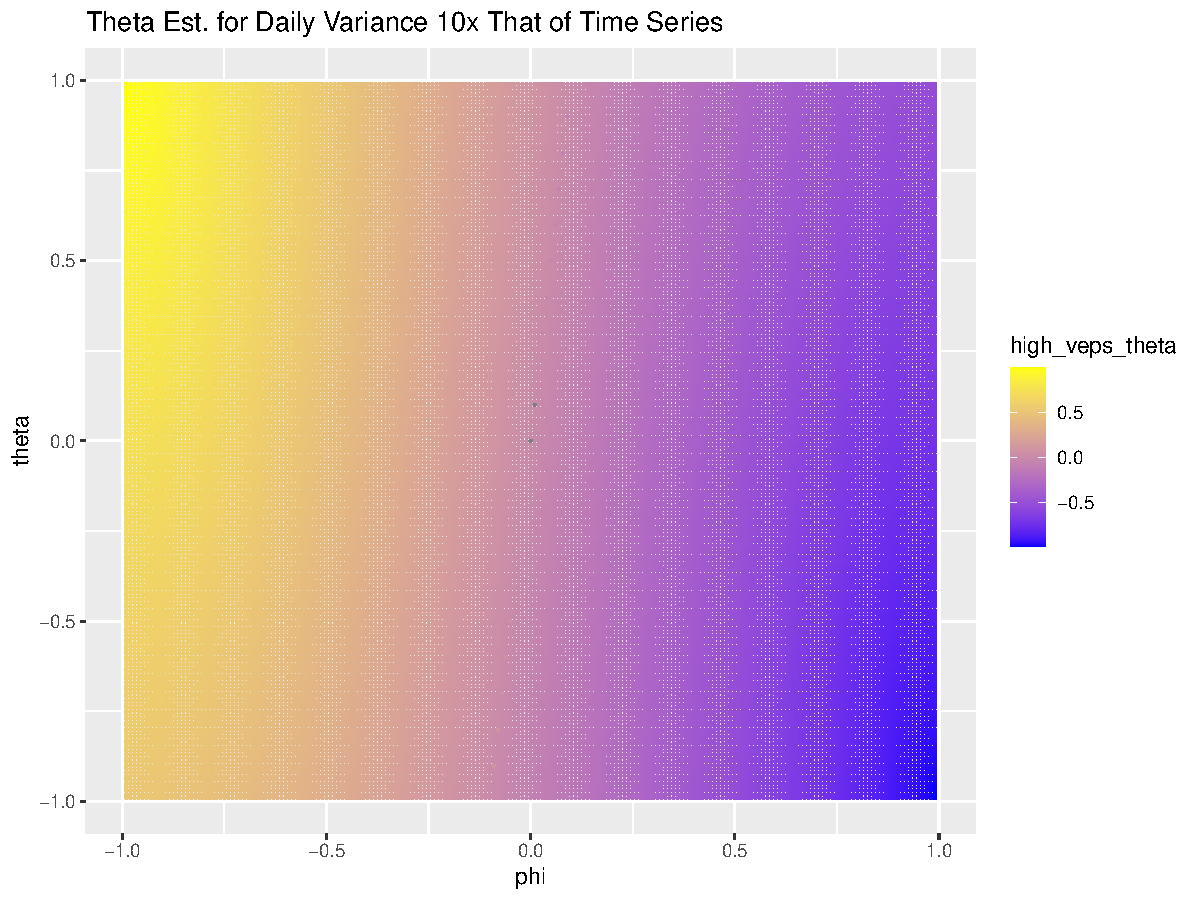
\includegraphics[width=0.48\textwidth]{images/output/high_veps.pdf}
%     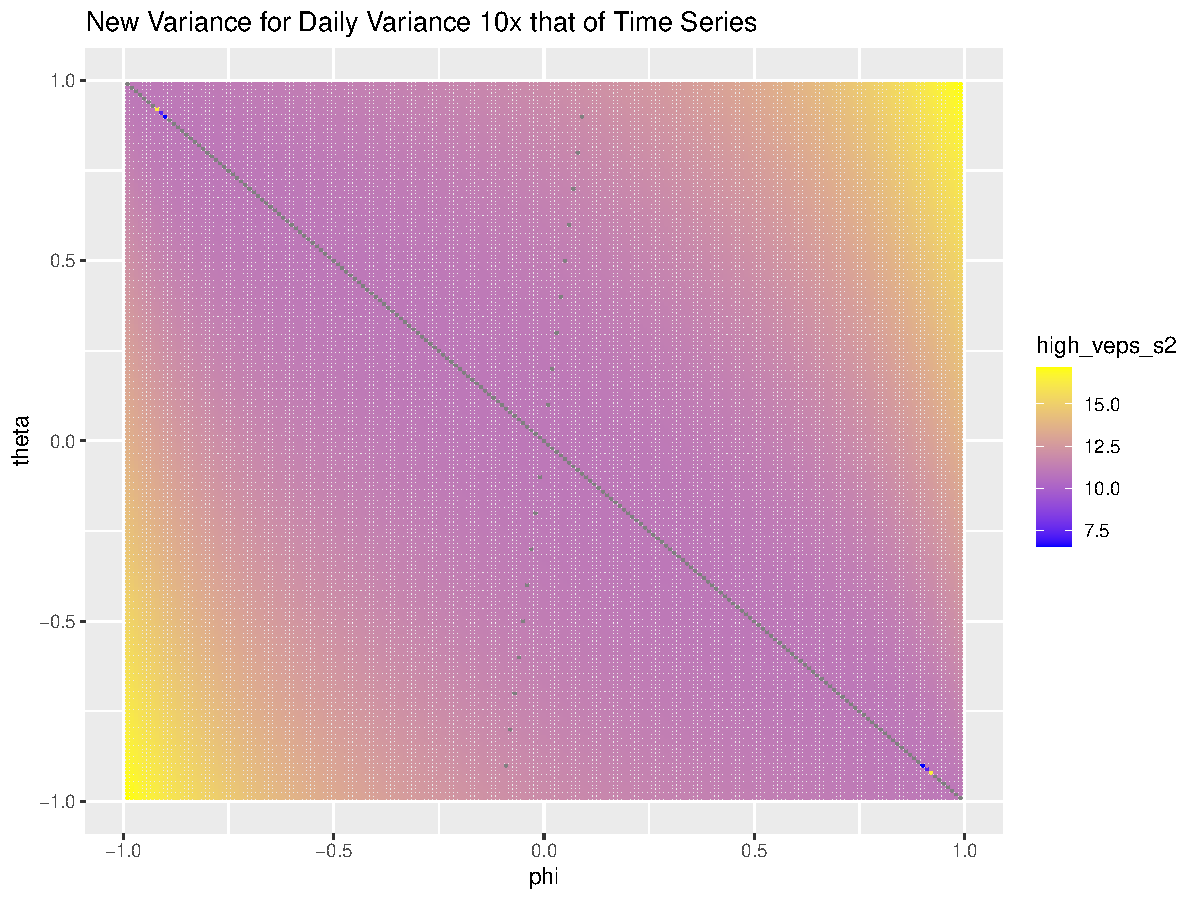
\includegraphics[width=0.48\textwidth]{images/output/high_veps_s2.pdf}

%     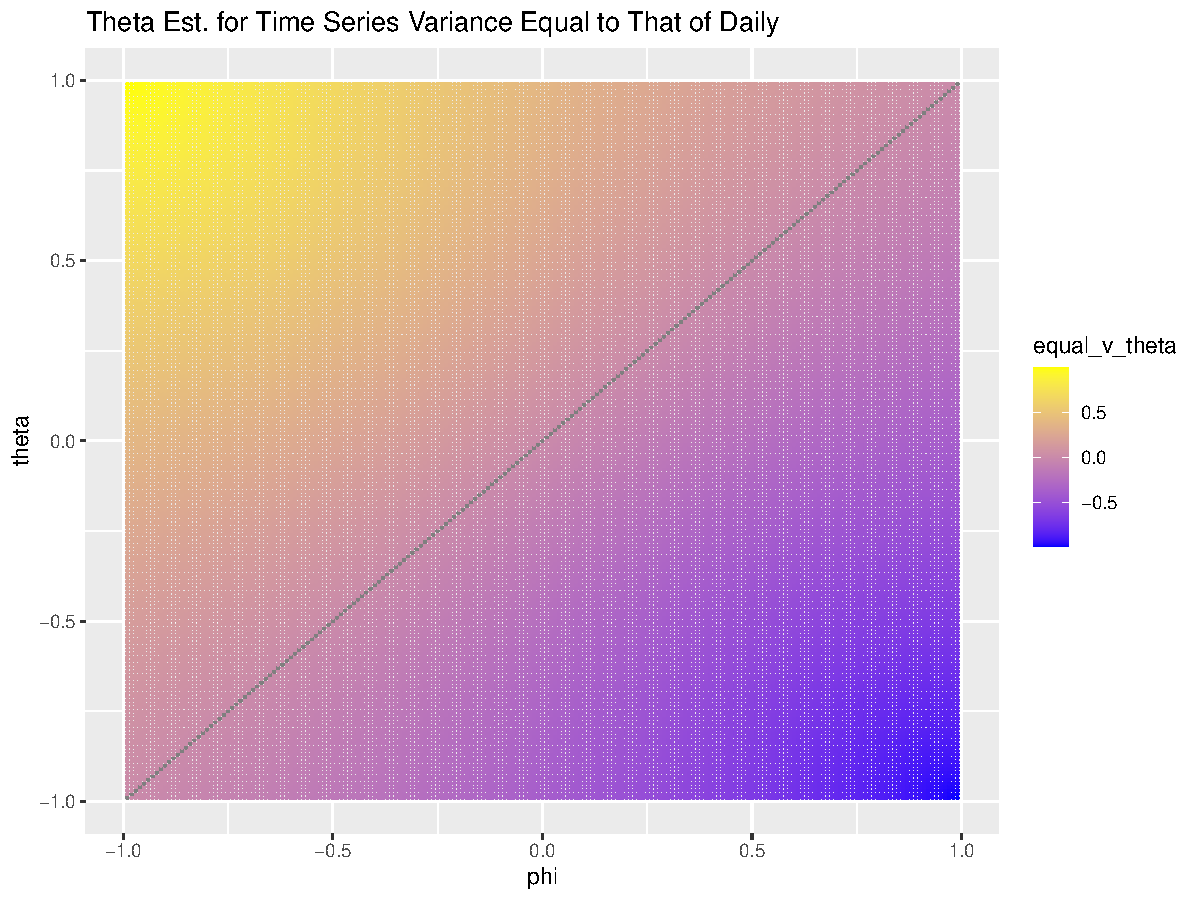
\includegraphics[width=0.48\textwidth]{images/output/equal_v.pdf}
%     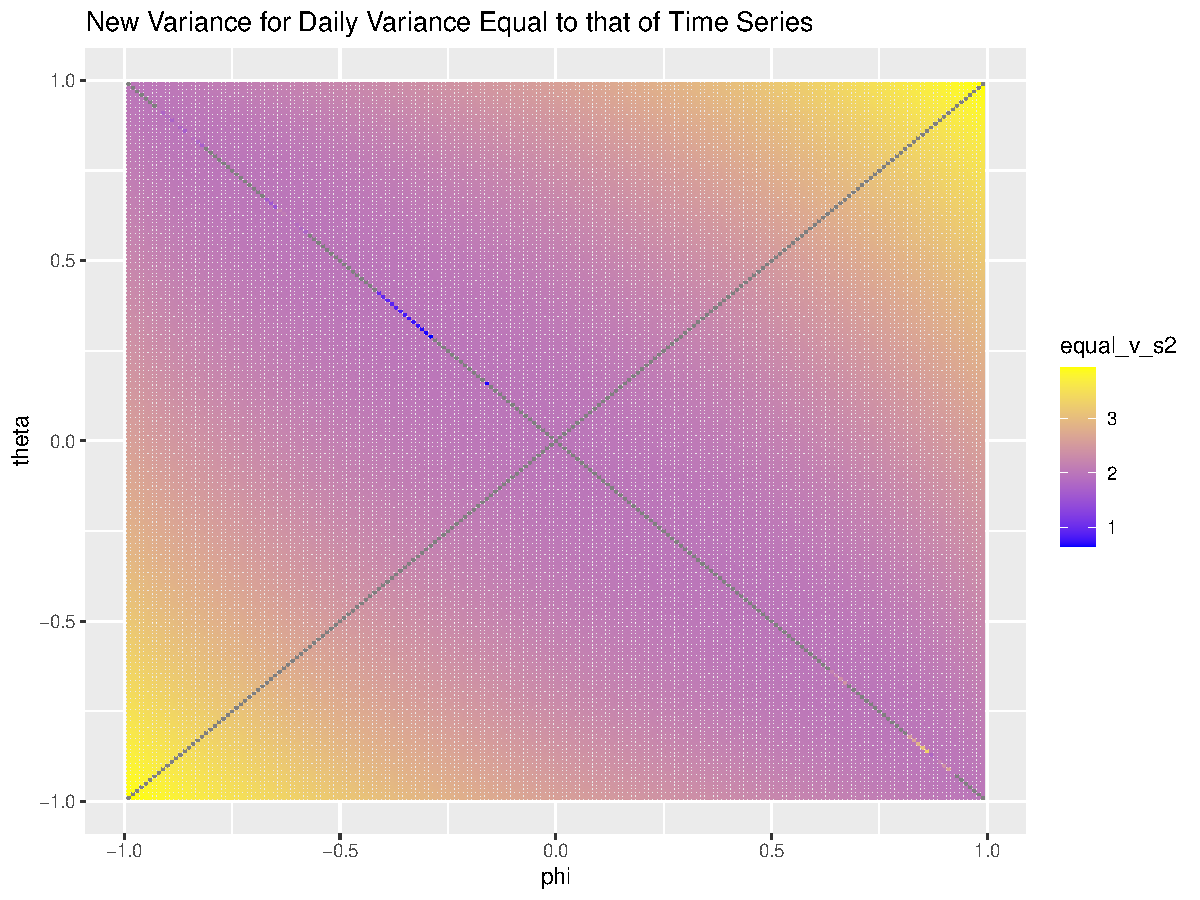
\includegraphics[width=0.48\textwidth]{images/output/equal_v_s2.pdf}

%     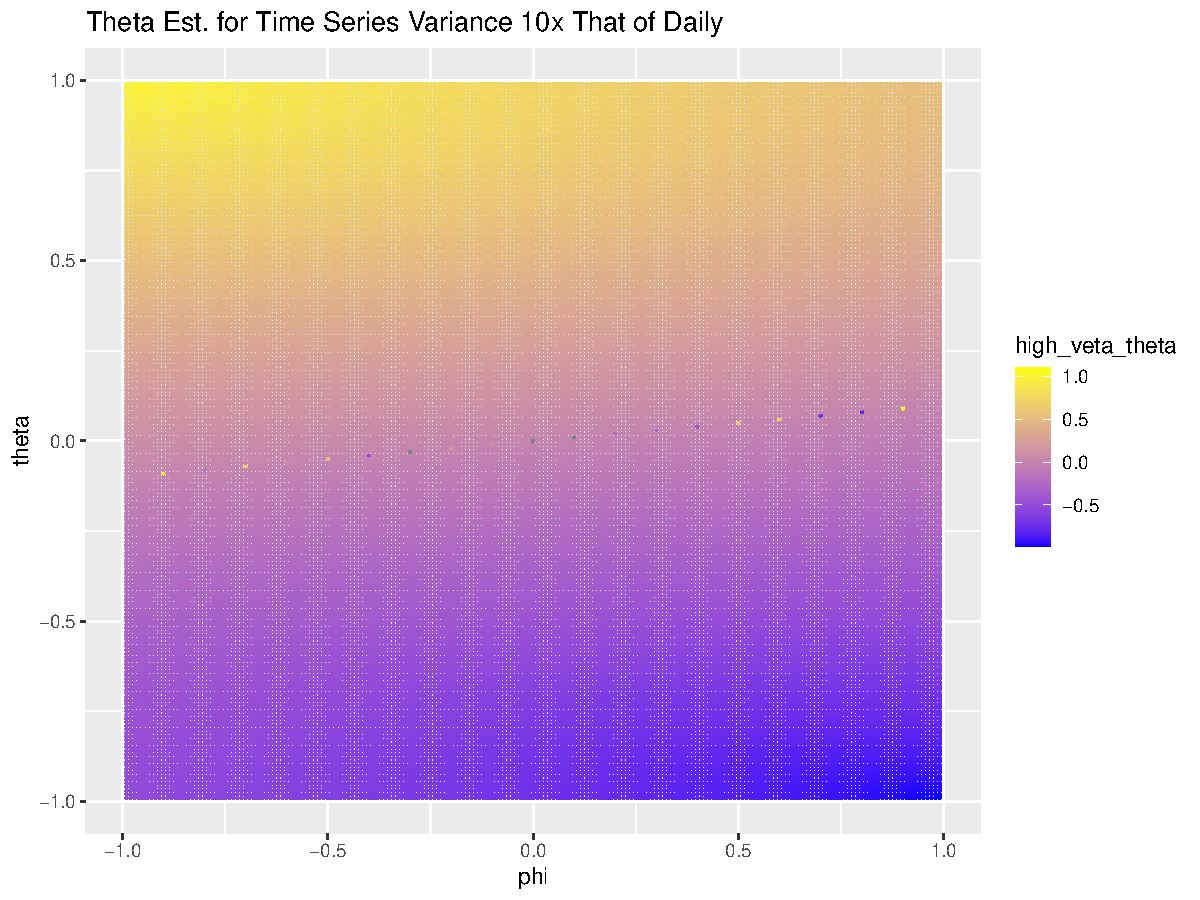
\includegraphics[width=0.48\textwidth]{images/output/high_veta.pdf}
%     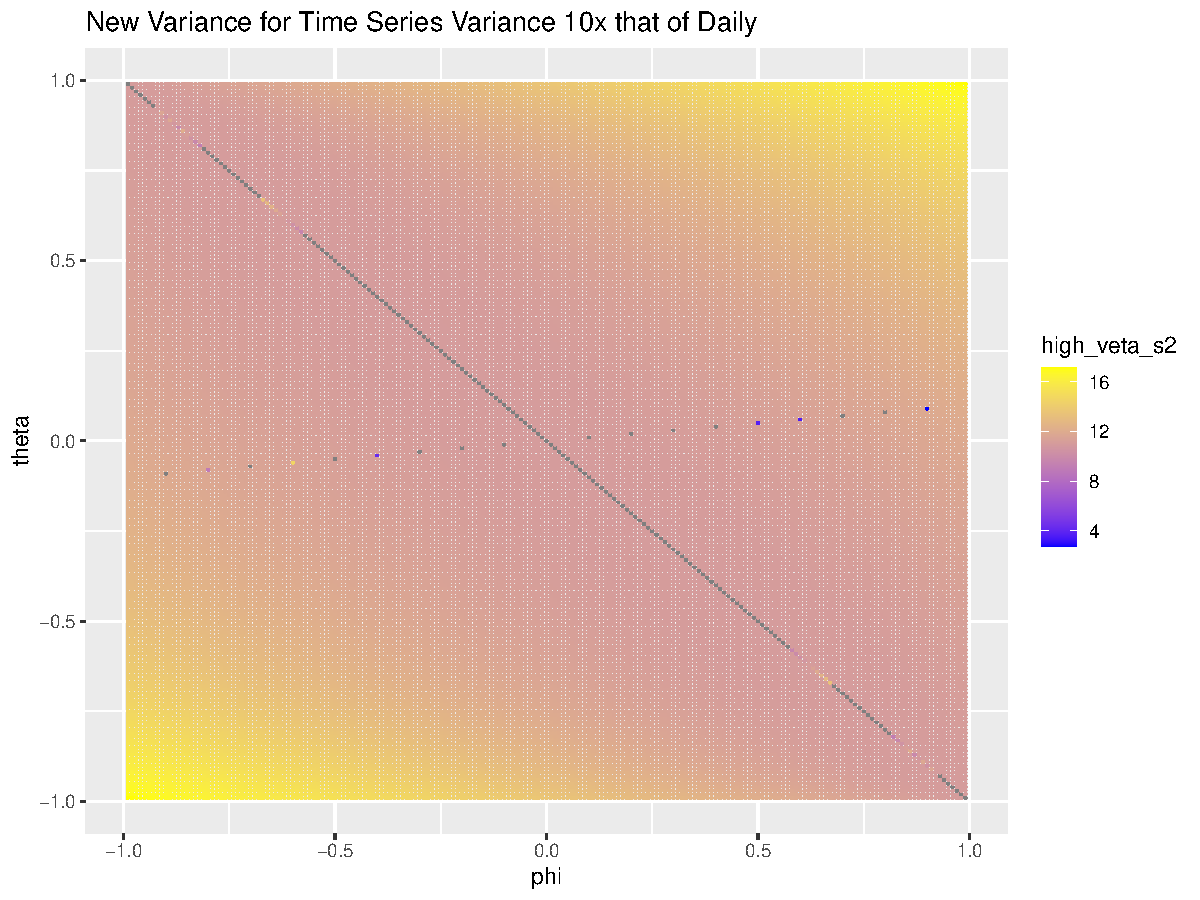
\includegraphics[width=0.48\textwidth]{images/output/high_veta_s2.pdf}

%     \caption{MA and Variance Parameters for ARMA-Noise model fit to ARMA(1,1)}
% \end{figure}
% \section{Reconfiguring Likelihood Function}

% We start with the following expression for the likelihood function $L(\xi|\mathbf{y})$:

% $$ L(\xi|\mathbf{y}) = (2\pi)^{-N/2}|\Omega|^{-1/2}\exp{(-\frac{1}{2})\mathbf{y}'\Omega^{-1}}\mathbf{y} $$

% $$ L_b(\xi_b|\mathbf{w}) = (2\pi)^{-N/2}|\Gamma_b|^{-1/2}\exp{(-\frac{1}{2})\mathbf{w}'\Gamma_b^{-1}}\mathbf{w} $$

% From Brockwell and Davis 1987, we can express the above equation as:

% $$ L(\phi,\theta_b,\sigma_b^2) = (2\pi\sigma_b^2)^{-T/2}(r_0...r_{T-1})^{-1/2}\exp{\left[ -\frac{1}{2}\sigma_b^2\sum_{j=1}^T(w_j -\hat{w}_j)^2/r_{j-1} \right]} $$

% This is based on applying the Innovations Algorithm (Proposition 5.2.2 from the same text). From this we get the following expressions for our maximum likelihood estimates:

% $$ \hat{\sigma}_b^2 = T^{-1} S(\hat{\phi}, \hat{\theta}) \qquad S(\hat{\phi}, \hat{\theta}) = \sum_{j=1}^T (w_j - \hat{w}_j)^2/r_{j-1} $$

% $$ l(\phi,\theta,\sigma_b^2|\mathbf{w}) = \frac{-T}{2}\text{ln}(2\pi\sigma_b^2) - \frac{1}{2}\sum_{j=0}^{T-1}\text{ln}(r_j) - \frac{1}{2}\sigma_b^{-2}\sum_{j=1}^T (w_j - \hat{w}_j)^2/r_{j-1}  $$

% $$ \frac{\partial l}{\partial \sigma_b^2} = -\frac{T}{2\sigma_b^2} + \frac{1}{2\sigma_b^4}\sum_{j=1}^T (w_j - \hat{w}_j)^2/r_{j-1}$$

% $$ \frac{\partial^2 l}{\partial \sigma_b^4} = \frac{T}{2\sigma_b^4} - \frac{1}{\sigma_b^6}\sum_{j=1}^T (w_j - \hat{w}_j)^2/r_{j-1}$$

% From 8.7.3 of Brockwell and Davis we obtain the expectation of the above expression, which we negate to find the Fischer Information:

% $$ I_{\sigma_b^2,\sigma_b^2} = -\mathbb{E}\left(\frac{\partial^2 l}{\partial \sigma_b^4}\right) = -\mathbb{E}\left(\frac{T}{2\sigma_b^4} - \frac{1}{\sigma_b^6}\sum_{j=1}^T (w_j - \hat{w}_j)^2/r_{j-1}\right) = \frac{T}{2\sigma_b^4} $$

% The relative simplicity of these derivative expressions are justified on page 256 of Brockwell and Davis, which states that $\{ (w_j-\hat{w_j})^2\}_{j=1}^T$ and $\{r_j\}_{j=1}^T$ are independent of $\sigma_b^2$.
% \bibliography{bib}

% In seeking the off-diagonal terms of the asymptotic variance matrix, we give the following expressions:

% \begin{equation}
%     \frac{\partial^2 l}{\partial \sigma_b^2 \partial \phi} = \frac{1}{2\sigma_b^4} \frac{\partial}{\partial \phi} \left[ \sum_{j=1}^T (w_j - \hat{w}_j)^2/r_{j-1}\right] 
%     \label{eq:fischer_phi}
% \end{equation}

% \begin{equation}
%     \frac{\partial^2 l}{\partial \sigma_b^2 \partial \theta_b} = \frac{1}{2\sigma_b^4} \frac{\partial}{\partial \theta_b} \left[ \sum_{j=1}^T (w_j - \hat{w}_j)^2/r_{j-1}\right] 
%     \label{eq:fischer_theta}
% \end{equation}

% For the simplification of calculations, we leverage the use of a transformed process: 
% $$v_t = \begin{cases}
%     \sigma_b^{-1}w_t & t = 1,...,m \\ \sigma_b^{-1}\phi(B)w_t & t > m 
    
% \end{cases} \qquad m = \text{max}(p,q)$$

% From page 177 we get: 
% $$ \begin{cases}
%     r_0 = (1 + 2\phi\theta_b + \theta_b^2)/(1-\phi^2), \\
%     \theta_{t} = \theta_b/r_{t-1}, \\
%     r_t = 1 + \theta_b^2 - \theta_b^2/r_{t-1}
    
% \end{cases} $$

% The one-step predictors given on page 176 then reduce to:
% $$\begin{cases}
    
%     \hat{w}_{t+1} = \phi w_t + \theta_{t}(w_t - \hat{w}_{t}) & n\geq m
% \end{cases}$$

% $$ \frac{\partial r_0}{\partial \phi} = \frac{2\theta_b(1-\phi^2) + (1 + 2\phi\theta_b + \theta_b^2)(2\phi)}{(1-\phi^2)^2}$$

% This is beginning to suggest that a closed form for the final two missing covariances will not be viable.

% Let's look at how the set $\{r_i\}$ develops for a few cases of $\phi$ and $\theta$:


% \begin{figure}[h]
%     \centering
%     \begin{minipage}[b]{0.45\textwidth}
%         \centering
%         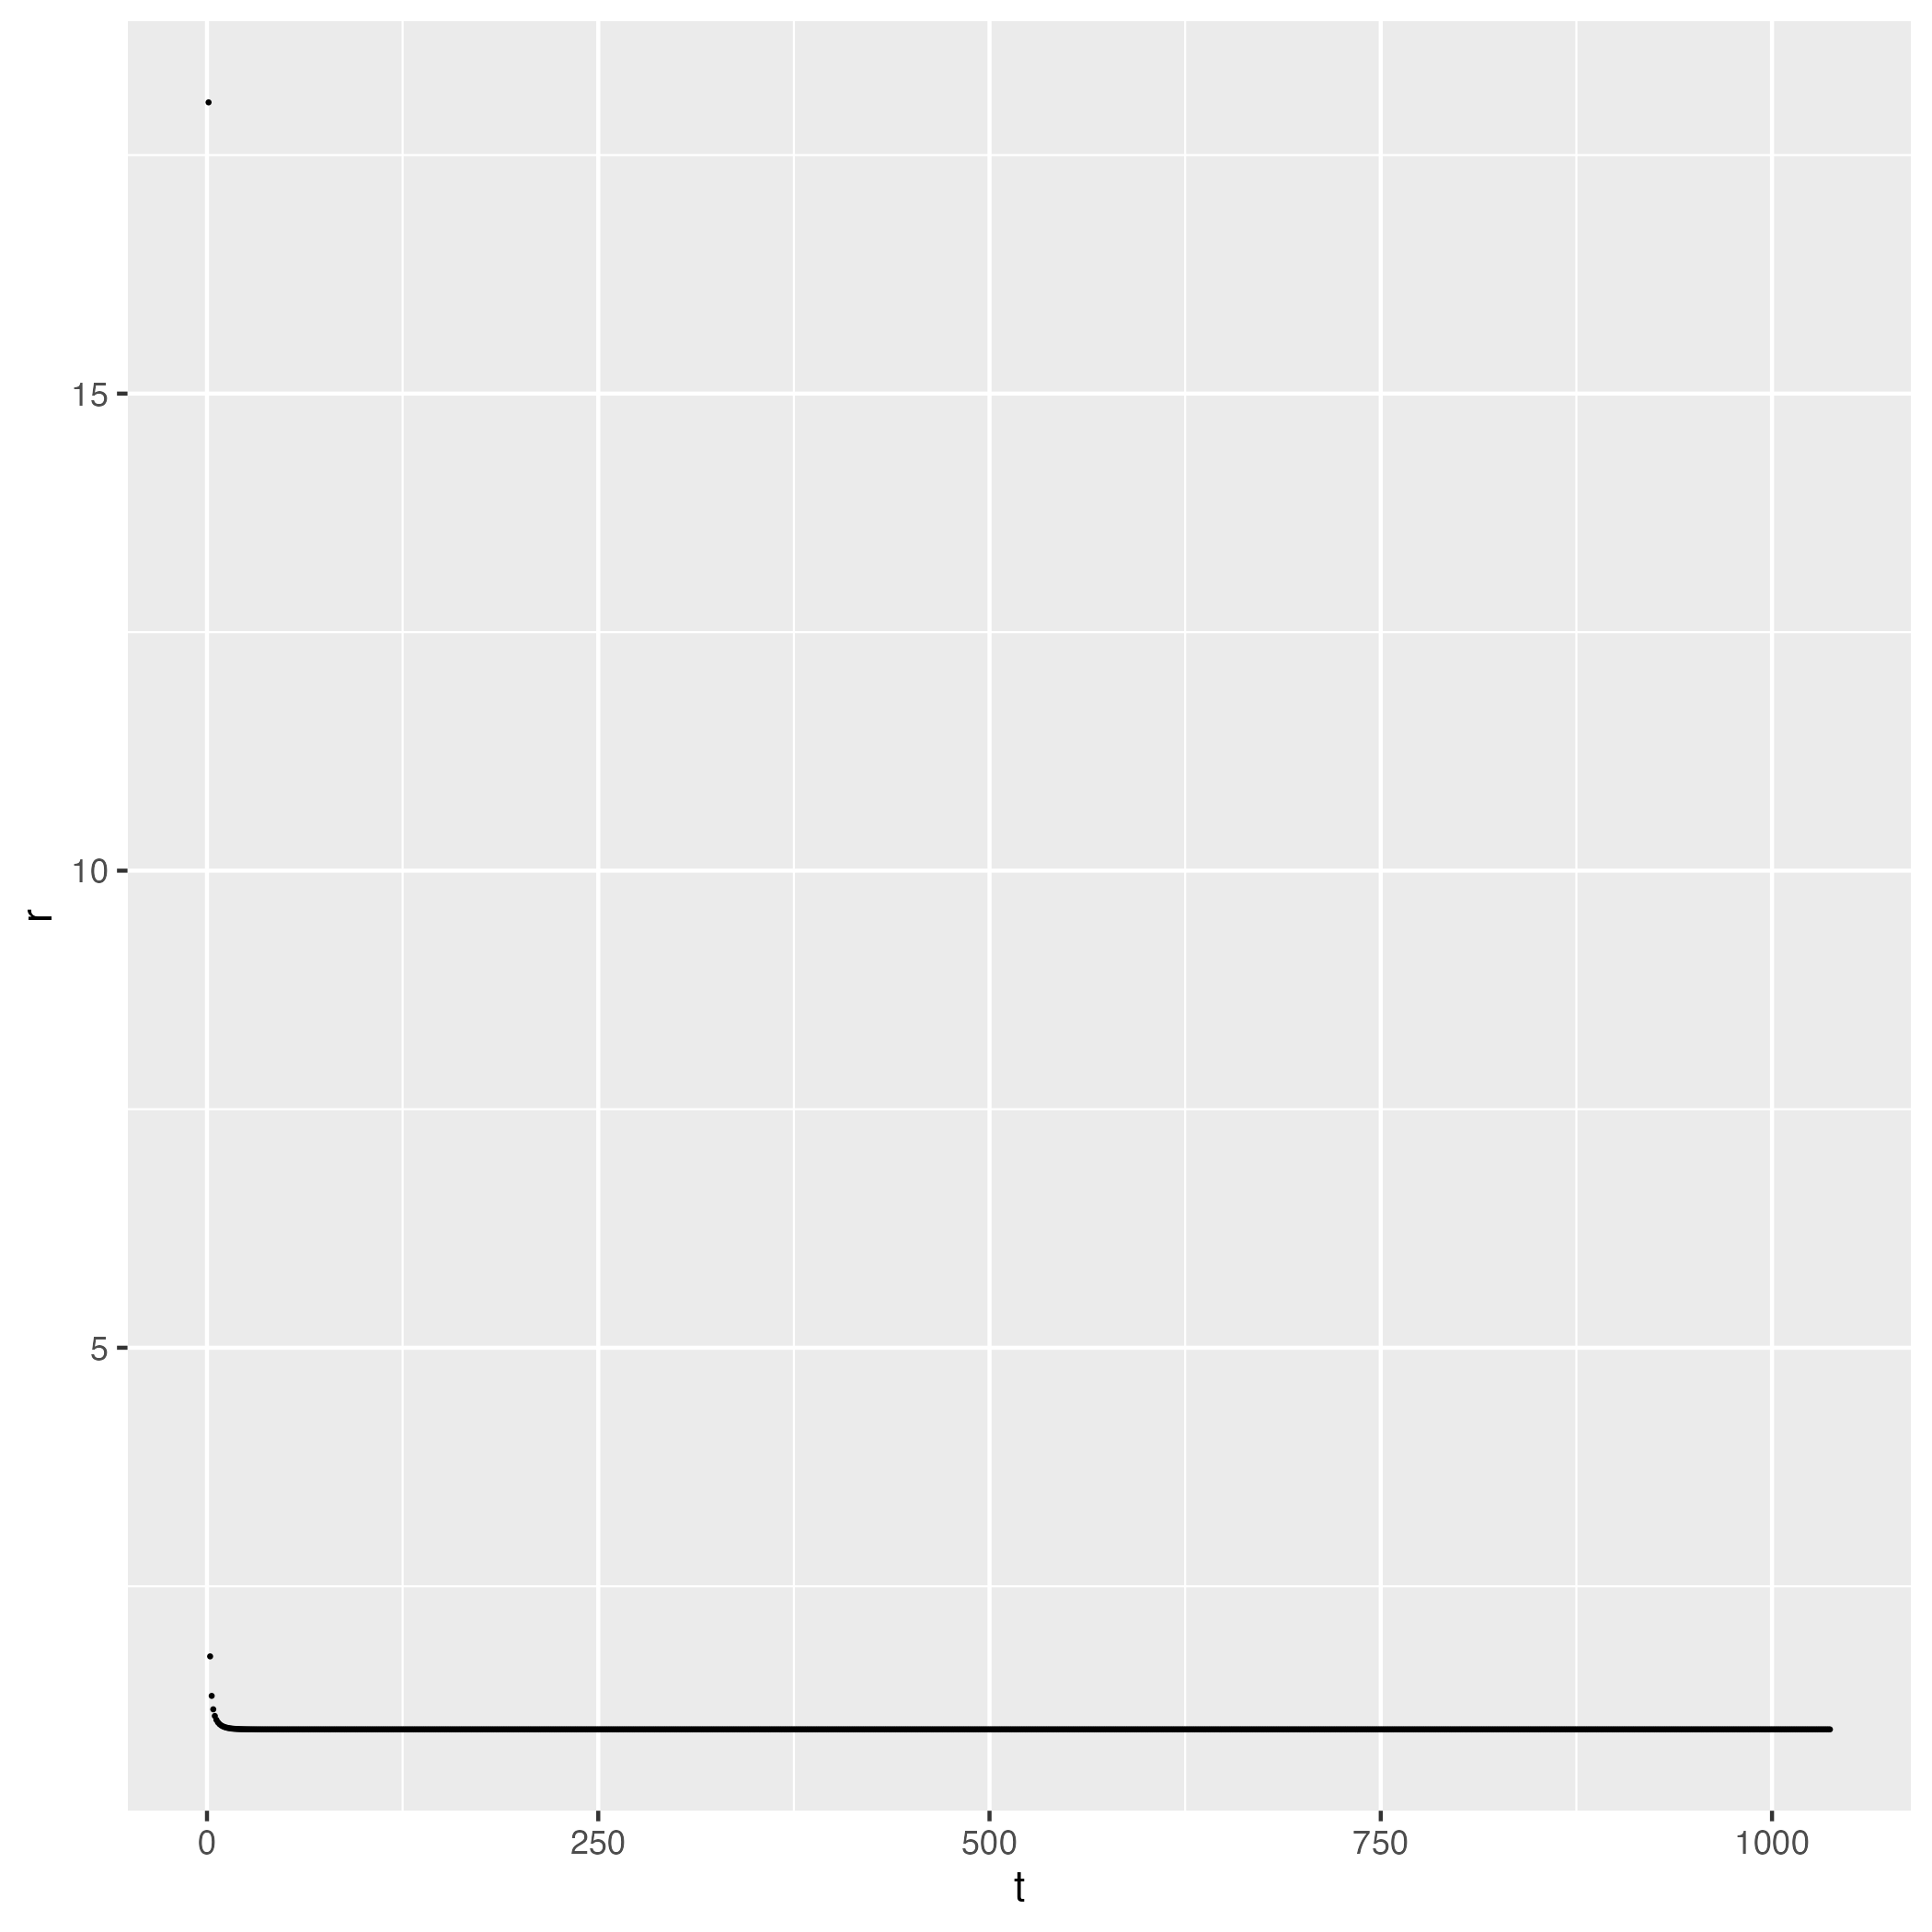
\includegraphics[width=\linewidth]{images/output/r_t.png}

%         \label{fig:image1}
%     \end{minipage}
%     \hfill
%     \begin{minipage}[b]{0.45\textwidth}
%         \centering
%         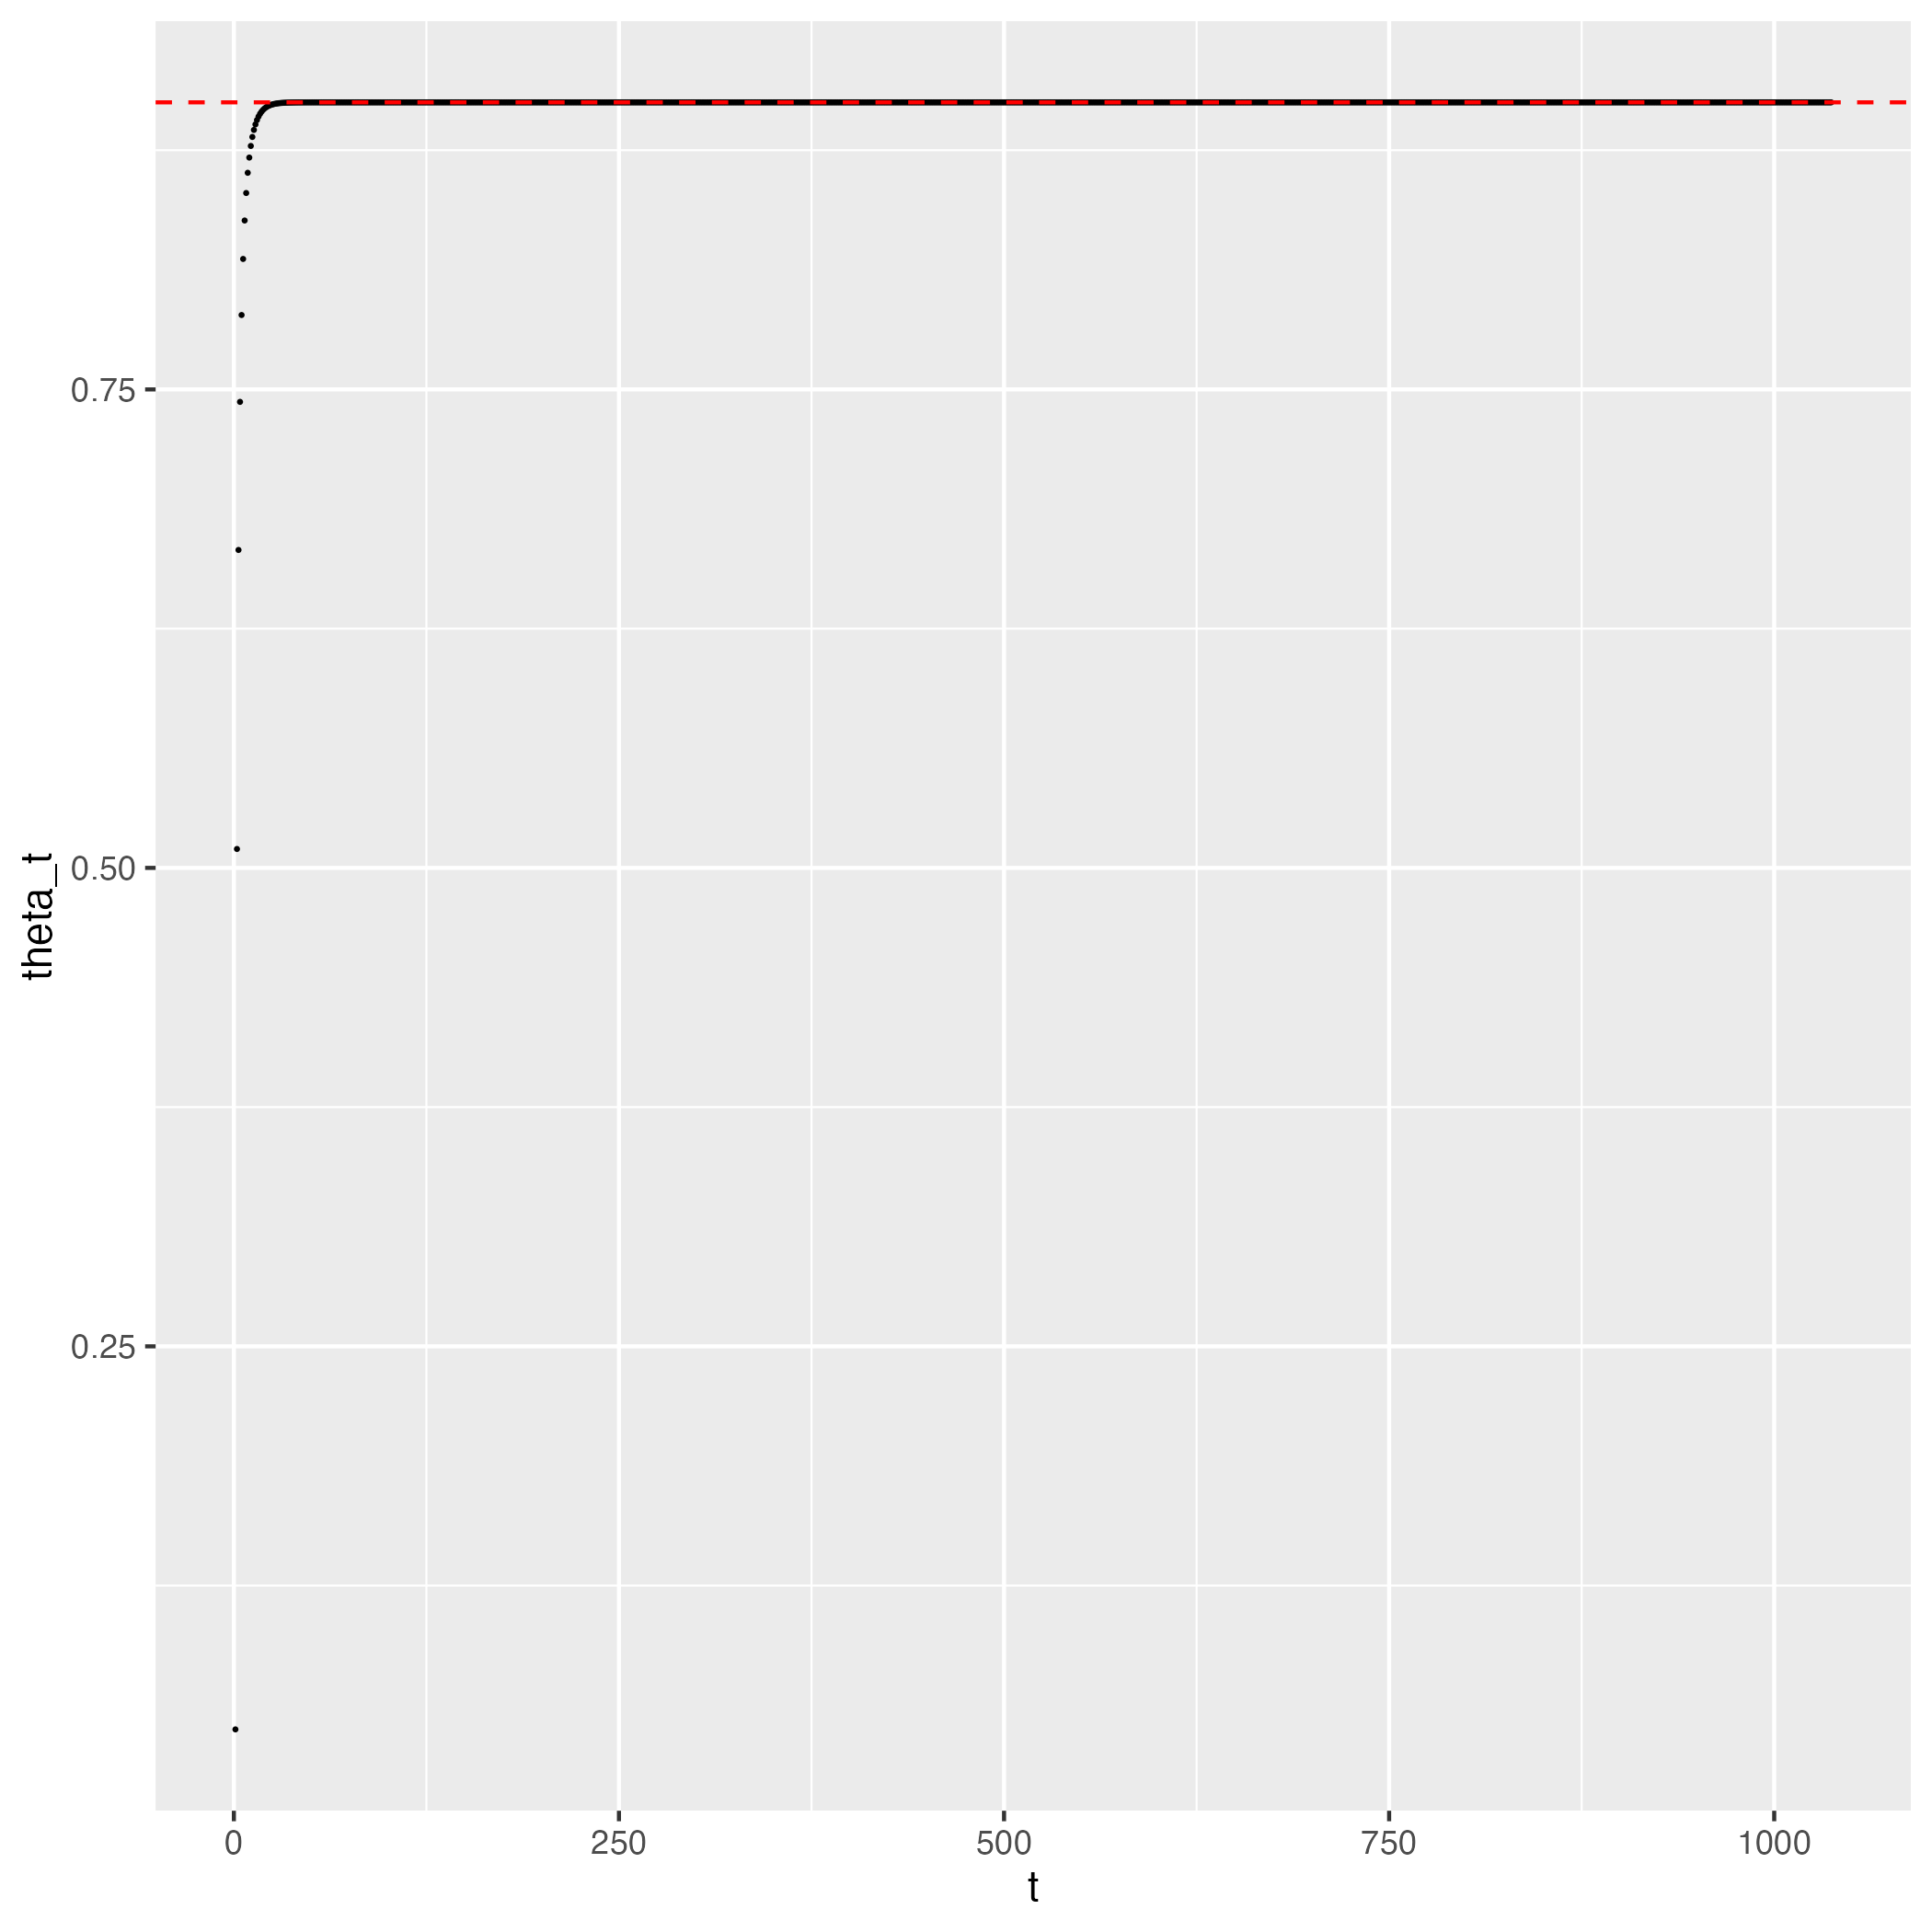
\includegraphics[width=\linewidth]{images/output/theta_t.png}

%         \label{fig:image2}
%     \end{minipage}
% \end{figure}

% Seeing how quickly $\{r_t\}$ and $\{\theta_t\}$ approach 1 and $\theta$, respectively, we're going to treat those as fixed values for now for the purposes of simplification. Equations \ref{eq:fischer_phi} and \ref{eq:fischer_theta} become: 

% $$ \frac{\partial}{\partial \phi}\frac{(w_j-\hat{w}_j)^2}{r_{j-1}} = (-2(w_j - \hat{w}_{j})(\frac{\partial}{\partial\phi}\hat{w}_{j})r_{j-1} - (w_j - \hat{w}_j)^2\frac{\partial}{\partial\phi}r_{j-1})r_{j-1}^{-2} $$

% $$ \frac{\partial \hat{w}_j}{\partial \phi} \approx w_{j-1} - \theta \frac{\partial}{\partial \phi} \hat{w}_{j-1} = w_{j-1} - \theta w_{j-2} + \theta^2 \frac{\partial}{\partial \phi} \hat{w}_{j-2} ... $$

% $$ \frac{\partial \hat{w}_j}{\partial \phi} \approx \sum_{i = 1}^{j-1}(-\theta)^{i-1}w_{j-i} $$

% $$ \frac{\partial \hat{w}_j}{\partial \theta} \approx \sum_{i=1}^{j-1}w_{n-i}[(-\theta)^{i-1} - (\phi + \theta)(i-1)(-\theta)^{i-2}] $$

% $$ I_{(\phi,\theta)} = \left[\begin{array}{cc}
%     (1 - \phi ^ 2) ^ {-1} & (1 + \phi \theta)^{-1}  \\
%     (1 + \phi \theta)^{-1}  & (1 - \theta ^ 2) ^ {-1}
% \end{array}\right] $$

% $$ \hat{w}_j \approx (\phi + \theta)\sum_{i=1}^{j-1}w_{j-i}(-\theta)^{i-1} $$

% $$ I_{\phi,\sigma_b^2} = -\sigma_b^{-4}\left[\sum_{j=1}^T\sum_{i=1}^{j-1}\sum_{k=1}^{j-1}(\phi + \theta)(-\theta)^{i + k - 2}\kappa(j-i,j-k) - \sum_{j=1}^T\sum_{i=1}^{j-1}(-\theta) ^{i-1}\kappa(j,j-i)\right] $$

% Because $\kappa(i,k) = 0, |i-k|>1$, this simplifies to:

% $$ I_{\phi,\sigma_b^2} = -\sigma_b^{-4}\left[(\phi + \theta)\sum_{j=2}^T\left[(1 + \theta^2)\sum_{i=1}^{j-2}(-\theta)^{2i-2} + 2\theta\sum_{i=1}^{j-2}(-\theta)^{2i-1} + \frac{1 + 2\phi\theta + \theta^2}{1-\phi^2}(-\theta)^{2j-4}\right] -T\theta\right]$$

% Let's define $a_i:=(-\theta)^{i-1} - (\phi + \theta)(i-1)(-\theta)^{i-2}$, then:
% $$ I(\theta,\sigma_b^2) = -\sigma_b^{-4}\sum_{j=1}^T\sum_{i=1}^{j-1}\sum_{k=1}^{j-1}\left[\frac{a_i\kappa(j,j-1)}{j-1} - (\phi + \theta)(-\theta)^{k-1}a_i\kappa(j-k,j-1)\right] $$

% This simplifies to:
% $$I(\theta,\sigma_b^2) = -\sigma_b^{-4}\left[(T-1)a_1\theta - (\phi + \theta)\sum_{j=2}^T \left[\sum_{i=1}^{j-2} \left\{a_i[(1 + \theta^2)(-\theta)^i + \theta(-\theta)^{i+1}] + a_{i+1}\theta(-\theta)^i\right\} + a_{j-1}\frac{1 + \phi\theta +\theta^2}{1 - \phi^2}(-\theta)^{j-1}\right] \right]$$


% $$ \kappa(i,j) = \begin{cases}
%     (1 + 2\phi\theta + \theta^2)/(1-\phi^2), & i=j=1, \\ 
%     1 + \theta^2, & i = j \geq 2, \\
%     \theta, & |i-j| = 1, \\
%     0, & \text{else.}
% \end{cases} $$

% \section{Misc. Pieces}
% \subsection{breakdown}
% Things currently break down if estimates for theta are very small
% \subsection{unnamed}
% If $\{w_t\}$ is an ARMA-Noise Process parameterized by $\phi,\theta,\sigma_\eta^2,\sigma_\varepsilon^2, n$, then its covariance matrix has the following spectral decomposition:

% \begin{equation}
%     \label{eq:X_t}
%     X_t = \left[ \begin{array}{cccc}
%         \mathbf{1}_n & \mathbf{0} & \dots & \mathbf{0} \\
%         \mathbf{0} & \mathbf{1}_n & \ddots & \vdots \\
%         \vdots & \ddots & \ddots & \mathbf{0} \\
%         \mathbf{0} & \dots & \mathbf{0}& \mathbf{1}_n 
%     \end{array} \right]
% \qquad
% X_t'X_t = nI_T
% \qquad
%     X_tX_t' = \left[ \begin{array}{cccc}
%         \mathbf{J}_n & \mathbf{0} & \dots & \mathbf{0} \\
%         \mathbf{0} & \mathbf{J}_n & \ddots & \vdots \\
%         \vdots & \ddots & \ddots & \mathbf{0} \\
%         \mathbf{0} & \dots & \mathbf{0}& \mathbf{J}_n 
%     \end{array} \right]
% \end{equation}

% \begin{equation}
%     \label{eq:cov_arman}
%     \Sigma_{\mathbf{w}} = \Sigma_\uu + \Sigma_\mathbf{a} = \sigma_\eta^2P\Lambda P' + \sigma_\varepsilon^2n^{-1}I = P(\sigma_\eta^2\Lambda + \sigma_\varepsilon^2n^{-1}I)P'
% \end{equation}


% $$\Sigma_{\hat{\uu}} = \Sigma_\uu X_t'\Sigma_\yy^{-1}X_t\Sigma_\uu = \sigma_\eta^4 \GG X_t' \Omega^{-1} X_t \GG$$ 

% Expanding with respective spectral decompositions yields:

% $$\Sigma_{\hat{\uu}} = \sigma_\eta^4 P \Lambda P'X_t' \left[\begin{array}{cc}
%     n^{-1/2}X_tP & Q  
% \end{array}\right] 
% \left[ \begin{array}{cc}
%     (n\sigma_\eta^2 \Lambda + \sigma_\varepsilon^2I)^{-1} & \mathbf{0} \\
%     \mathbf{0} & \sigma_\varepsilon^{-2}I
% \end{array} \right] \left[ \begin{array}{cc}
%     n^{-1/2}P'X_t'  \\
%     Q' 
% \end{array} \right] X_t'P\Lambda P'
% $$

% Leveraging the orthogonality among column vectors of $X_tP$ and $Q$, we obtain:

% $$ \Sigma_{\hat{\uu}} = \sigma_\eta^4   \left[\begin{array}{cc}
%     n^{1/2}P\Lambda & \mathbf{0}  
% \end{array}\right] 
% \left[ \begin{array}{cc}
%     (n\sigma_\eta^2 \Lambda + \sigma_\varepsilon^2I)^{-1} & \mathbf{0} \\
%     \mathbf{0} & \sigma_\varepsilon^{-2}I
% \end{array} \right] \left[ \begin{array}{cc}
%     n^{1/2}\Lambda P'  \\
%     \mathbf{0}
% \end{array} \right] 
%  $$

%  After simplifying we finally obtain:

%  $$ \Sigma_{\hat{\uu}} = \sigma_\eta^4   \left[\begin{array}{cc}
%     n^{1/2}P\Lambda  
% \end{array}\right] 
% \left[ \begin{array}{cc}
%     (n\sigma_\eta^2 \Lambda + \sigma_\varepsilon^2I)^{-1} 
% \end{array} \right] \left[ \begin{array}{cc}
%     n^{1/2}\Lambda P'  
% \end{array} \right]  =  
%     P \Lambda_* P', \qquad (\Lambda_*)_{i,j} = \begin{cases}
%         \frac{\sigma_\eta^4\lambda_i^2}{\sigma_\eta^2\lambda_i + \sigma_\varepsilon^2/n} & i=j \\
%         0 & i \neq j
%     \end{cases}   
%  $$

 


% \bibliography{bib}

